%\documentclass[]{article}
\documentclass[11pt]{article}
\usepackage[usenames,dvipsnames]{xcolor}

\usepackage[T1]{fontenc}
%\usepackage{lmodern}
\usepackage{tgtermes}
\usepackage{amssymb,amsmath}
%\usepackage[margin=1in]{geometry}
\usepackage[letterpaper,bottom=1in,top=1in,right=1.25in,left=1.25in,includemp=FALSE]{geometry}
\usepackage{pdfpages}
\usepackage[small]{caption}

\usepackage{ifxetex,ifluatex}
\usepackage{fixltx2e} % provides \textsubscript
% use microtype if available
\IfFileExists{microtype.sty}{\usepackage{microtype}}{}
\ifnum 0\ifxetex 1\fi\ifluatex 1\fi=0 % if pdftex
\usepackage[utf8]{inputenc}
\else % if luatex or xelatex
\usepackage{fontspec}
\ifxetex
\usepackage{xltxtra,xunicode}
\fi
\defaultfontfeatures{Mapping=tex-text,Scale=MatchLowercase}
\newcommand{\euro}{€}
\fi
%

\usepackage{fancyvrb}

\usepackage{ctable,longtable}

\usepackage[section]{placeins}
\usepackage{float} % provides the H option for float placement
\restylefloat{figure}
\usepackage{dcolumn} % allows for different column alignments
\newcolumntype{.}{D{.}{.}{1.2}}

\usepackage{booktabs} % nicer horizontal rules in tables

%Assume we want graphics always
\usepackage{graphicx}
% We will generate all images so they have a width \maxwidth. This means
% that they will get their normal width if they fit onto the page, but
% are scaled down if they would overflow the margins.
%% \makeatletter
%% \def\maxwidth{\ifdim\Gin@nat@width>\linewidth\linewidth
%%   \else\Gin@nat@width\fi}
%% \makeatother
%% \let\Oldincludegraphics\includegraphics
%% \renewcommand{\includegraphics}[1]{\Oldincludegraphics[width=\maxwidth]{#1}}
\graphicspath{{.}{../Soccom_Code/socom_2013/}}


%% \ifxetex
%% \usepackage[pagebackref=true, setpagesize=false, % page size defined by xetex
%% unicode=false, % unicode breaks when used with xetex
%% xetex]{hyperref}
%% \else
\usepackage[pagebackref=true, unicode=true, bookmarks=true, pdftex]{hyperref}
% \fi


\hypersetup{breaklinks=true,
  bookmarks=true,
  pdfauthor={Christopher Grady, Rebecca Wolfe, Danjuma Dawop, and Lisa Inks},
  pdftitle={Promoting Peace Amidst Group Conflict: An Intergroup Contact Field Experiment in Nigeria},
  colorlinks=true,
  linkcolor=BrickRed,
  citecolor=blue, %MidnightBlue,
  urlcolor=BrickRed,
  % urlcolor=blue,
  % linkcolor=magenta,
  pdfborder={0 0 0}}

%\setlength{\parindent}{0pt}
%\setlength{\parskip}{6pt plus 2pt minus 1pt}
\usepackage{parskip}
\setlength{\emergencystretch}{3em}  % prevent overfull lines
\providecommand{\tightlist}{%
  \setlength{\itemsep}{0pt}\setlength{\parskip}{0pt}}

%% Insist on this.
\setcounter{secnumdepth}{2}

\VerbatimFootnotes % allows verbatim text in footnotes

\title{Promoting Peace Amidst Group Conflict: An Intergroup Contact Field
Experiment in Nigeria}

\author{
Christopher Grady, Rebecca Wolfe, Danjuma Dawop, and Lisa Inks
}


\date{December 10, 2019}


\usepackage{versions}
\makeatletter
\renewcommand*\versionmessage[2]{\typeout{*** `#1' #2. ***}}
\renewcommand*\beginmarkversion{\sffamily}
  \renewcommand*\endmarkversion{}
\makeatother

\excludeversion{comment}

%\usepackage[margins=1in]{geometry}

\usepackage[compact,bottomtitles]{titlesec}
%\titleformat{ ⟨command⟩}[⟨shape⟩]{⟨format⟩}{⟨label⟩}{⟨sep⟩}{⟨before⟩}[⟨after⟩]
\titleformat{\section}[hang]{\Large\bfseries}{\thesection}{.5em}{\hspace{0in}}[\vspace{-.2\baselineskip}]
\titleformat{\subsection}[hang]{\large\bfseries}{\thesubsection}{.5em}{\hspace{0in}}[\vspace{-.2\baselineskip}]
%\titleformat{\subsubsection}[hang]{\bfseries}{\thesubsubsection}{.5em}{\hspace{0in}}[\vspace{-.2\baselineskip}]
\titleformat{\subsubsection}[hang]{\bfseries}{\thesubsubsection}{1ex}{\hspace{0in}}[\vspace{-.2\baselineskip}]
\titleformat{\paragraph}[runin]{\bfseries\itshape}{\theparagraph}{1ex}{}{\vspace{-.2\baselineskip}}
%\titleformat{\paragraph}[runin]{\itshape}{\theparagraph}{1ex}{}{\vspace{-.2\baselineskip}}

%%\titleformat{\subsection}[hang]{\bfseries}{\thesubsection}{.5em}{\hspace{0in}}[\vspace{-.2\baselineskip}]
%%%\titleformat*{\subsection}{\bfseries\scshape}
%%%\titleformat{\subsubsection}[leftmargin]{\footnotesize\filleft}{\thesubsubsection}{.5em}{}{}
%%\titleformat{\subsubsection}[hang]{\small\bfseries}{\thesubsubsection}{.5em}{\hspace{0in}}[\vspace{-.2\baselineskip}]
%%\titleformat{\paragraph}[runin]{\itshape}{\theparagraph}{1ex}{}{\vspace{-.5\baselineskip}}

%\titlespacing*{ ⟨command⟩}{⟨left⟩}{⟨beforesep⟩}{⟨aftersep⟩}[⟨right⟩]
\titlespacing{\section}{0pc}{1.5ex plus .1ex minus .2ex}{.5ex plus .1ex minus .1ex}
\titlespacing{\subsection}{0pc}{1.5ex plus .1ex minus .2ex}{.5ex plus .1ex minus .1ex}
\titlespacing{\subsubsection}{0pc}{1.5ex plus .1ex minus .2ex}{.5ex plus .1ex minus .1ex}



%% These next lines tell latex that it is ok to have a single graphic
%% taking up most of a page, and they also decrease the space around
%% figures and tables.
\renewcommand\floatpagefraction{.9}
\renewcommand\topfraction{.9}
\renewcommand\bottomfraction{.9}
\renewcommand\textfraction{.1}
\setcounter{totalnumber}{50}
\setcounter{topnumber}{50}
\setcounter{bottomnumber}{50}
\setlength{\intextsep}{2ex}
\setlength{\floatsep}{2ex}
\setlength{\textfloatsep}{2ex}



\begin{document}
\VerbatimFootnotes

%\begin{titlepage}
%  \maketitle
%\vspace{2in}
%
%\begin{center}
%  \begin{large}
%    PROPOSAL WHITE PAPER
%
%BAA 14-013
%
%Can a Hausa Language Television Station Change Norms about Violence in Northern Nigeria? A Randomized Study of Media Effects on Violent Extremism
%
%Jake Bowers
%
%University of Illinois @ Urbana-Champaign (jwbowers@illinois.edu)
%
%\url{http://jakebowers.org}
%
%Phone: +12179792179
%
%Topic Number: 1
%
%Topic Title: Identity, Influence and Mobilization
%
%\end{large}
%\end{center}
%\end{titlepage}

\maketitle

\hypertarget{introduction}{%
\section{Introduction}\label{introduction}}

How can groups in conflict improve intergroup relations? Violent group
conflict has caused 2 million deaths since the year 2000 (Sundberg and
Melander 2013), forcibly displaced over 70 million people from their
homes in 2018 (UNHCR 2019), threatens food supplies in numerous
countries (Verwimp and others 2012), and extracts a psychological toll
on participants and victims (Schomerus and Rigterink 2018). Intergroup
animosity perpetuates conflict long after the original grievance is
immaterial or forgotten (Deutsch 1973; McDonnel 2017; Tajfel and Turner
1979), so improving intergroup relations is vital to stem the human,
economic, social, and psychological costs of violent group conflict.

Scholars and policymakers/practitioners consider \emph{cooperative}
intergroup contact -- contact in which members of two groups work
together to achieve common goals -- to be one of the most effective
tools for improving intergroup relations.\footnote{We will use the term
  \emph{cooperative contact} to refer to contact that meets Allport's
  conditions. Cooperative contact stands in contrast to other forms of
  incidental or unstructured contact that may not have positive effects
  on intergroup relations.} The hypothesis that cooperative contact
improves intergroup relations, known as the contact hypothesis (Allport
1954), motivates many policy interventions, from integrated public
housing (Deutsch and Collins 1951) and college dorms (Marmaros and
Sacerdote 2006) to workplace and school desegregation (Cook 1985; Cook,
Wrightsman, and Wrightsman 1971; Rao 2019). The contact hypothesis also
increasingly motivates peacebuilding programs (Ditlmann, Samii, and
Zeitzoff 2017; Lemmer and Wagner 2015). Through these types of
interventions, intergroup contact has improved relations between white
people and black people in the U.S. and South Africa (Burns, Corno, and
La Ferrara 2015; Carrell, Hoekstra, and West 2015; Marmaros and
Sacerdote 2006), Christians and Muslims in Iraq and Nigeria (Mousa 2018;
Scacco and Warren 2018), Jews and Arabs in Israel/Palestine (Ditlmann
and Samii 2016; Weiss 2019; Yablon 2012), and Hindus and Muslims in
India (Barnhardt 2009).

Despite these successes, scholars know little about the effects of
intergroup contact for groups engaged in a violent conflict. Cooperative
intergroup contact has only recently been tested in the field with
groups who have a recent history of violence (Lemmer and Wagner 2015;
Paluck, Green, and Green 2019), and never programatically with
communities who are perpetrating violence against each other. If one of
the goals of cooperative contact is to mitigate violent conflict,
interventions based on cooperative contact must be tested between groups
in a violent conflict.

Historical and ongoing violence poses the most difficult test for
contact and could interfere with mechanisms through which contact
improves relations. Scholars theorize that contact improves relations
mainly through providing information that dispels stereotypes,
increasing empathy and perspective-taking, reducing anxiety about
interacting with outgroup members, and making salient a superordinate
identity that includes both groups (Broockman and Kalla 2016; Dovidio et
al. 2017; Gaertner and Dovidio 2014; Page-Gould, Mendoza-Denton, and
Tropp 2008; Pettigrew and Tropp 2008). These mechanisms assume that
negative attitudes result from unfamiliarity, and that ``familiarity
breed{[}s{]} liking'' (Pettigrew and Tropp 2006, 766). We posit that
familiarity through cooperative contact allows groups to identify their
latent shared interests. By obscuring shared interests and highlighting
and reinforcing group differences, violent conflict could dull, prevent,
or even reverse the predicted positive effects of contact. For these
reasons, some scholars believe group reconciliation cannot begin until
conflict is resolved (Bar-Tal 2000).

Moreover, cooperative contact between some ingroup members and some
outgroup members can only meaningfully improve group relations under two
conditions. First, group members must generalize their positive
attitudes to the outgroup as a whole, not just the outgroup members with
whom the ingroup members interacted. Attitudes generalize when the
outgroup members involved in contact are viewed as typical of the
outgroup (Hewstone 1996). Second, effects of contact must diffuse to
other ingroup members. Diffusion can occur through the knowledge that
other ingroup members had positive contact with outgroup members (Wright
et al. 1997) or through changing social norms about cross-group
interaction (Christ et al. 2014; Paluck 2009). In contexts of historical
or ongoing violence, any cross-group interaction may mark an outgroup
member as atypical, and social norms may stay staunchly opposed to
intergroup cooperation.

Despite these reasons for caution, there are reasons to expect
cooperative contact to improve intergroup relations even in contexts of
ongoing violence. Contact should improve relations when there exists
shared group interests. Even in contexts of group violence, it is often
in each group's shared interest to reach a peaceful compromise because
fighting is costly (Fearon 1995). Cooperative contact to achieve a
common goal provides groups with an example of cooperation towards a
shared interest, and that experience can make groups imagine future
interactions for shared benefit. Cooperative contact can also remove the
psychological barriers to identifying shared interests, such as
stereotypes and feelings of threat and anxiety. Lastly, cooperation in
that benefits the group should generate group pressure to cooperate,
thus creating cooperative social norms.

To learn about whether cooperative contact can improve intergroup
relations amidst violent group conflict, we conducted a field experiment
with conflicting farmer and pastoralist communities in Nigeria. More
than an occupational difference, farmers who cultivate crops and
pastoralists who graze cattle define a major social cleavage in many
parts of the world. These groups conflict over land rights, which define
both of their livelihoods. Farmer-pastoralist conflict has escalated
throughout the Sahel in recent years, and nowhere more than in Nigeria.
The most recent conflict escalation has caused 7,000 deaths from
2014-2019, displaced hundreds of thousands of people from their homes,
and costs \$13 billion annually in lost economic productivity (Akinwotu
2018; Daniel 2018; Harwood 2019; McDougal et al. 2015). In our sample,
members of each community had been killed by members of the other
community within the year before the project began. Past and present
violence, occupational and ethnic differences, and fighting over
resources necessary for livelihoods all make this context a hard test
for contact theory.

We randomly assigned communities with ongoing farmer-pastoralist
violence to receive a contact-based intervention or serve as a control
group. The intervention formed mixed-group committees and provided them
with funds to build infrastructure that would benefit both communities;
committees then collaboratively chose and constructed infrastructure
projects.\footnote{The communities built boreholes, market stalls,
  primary health care facilities, etc.} The program also provided
mediation training to each community's leaders and held forums where the
groups discussed the underlying drivers of conflict. To measure the
effects of the intervention, we conducted pre- and post-intervention
surveys, a post-intervention natural public goods behavioral
game,\footnote{In a public goods game (PGG), research subjects are given
  money and told they can keep the money or donate it to a public fund.
  Money donated to the public fund is multiplied by some amount and then
  shared with all subjects. Our PGG is \emph{natural} because it was
  conducted in a natural setting, rather than a lab. The funding for the
  PGG came from the National Science Foundation under Grant No.~1656871.}
and twelve months of systematic observations in markets and social
events during the intervention.

We find that the program increased intergroup contact, intergroup trust,
and perceptions of physical security. We see signs of the positive
effects in fieldwork as well as in data -- in one of the treatment
sites, farmers defended pastoralists from a group of anti-pastoralist
vigilantes, rather than assist the vigilantes in removing the
pastoralists and claiming their land. Our results also show that the
intervention affected communities as a whole, not just community members
directly involved in the intergroup contact. Individuals who directly
engaged in intergroup contact changed the most positively from baseline
to endline, but we also observe positive spillovers of trust to group
members for whom we did not exogenously increase intergroup contact.

This study expands our knowledge about group conflict in several ways.
First, this study teaches us about the capacity of intergroup contact to
improve intergroup relations and reduce conflict. Peacebuilding
organizations implement numerous contact-based interventions in violent
contexts each year, but its efficacy to improve intergroup attitudes
amid real-world conflict is an open question (Ditlmann, Samii, and
Zeitzoff 2017; Paluck, Green, and Green 2019). To our knowledge this is
the first field experimental test of a contact-based intervention
implemented during an active conflict. The results suggest that
contact-based peacebuilding programs can effectively improve
relationships between conflicting groups and is especially relevant to
conflict resolution in the cases of intergroup and intercommunal
conflicts.

Second, we contribute to the literature about informal structures, such
as social norms, in solving collective action problems. Conflict between
farmers and pastoralists is a collective action problem in that both
groups would be materially better off avoiding violence through
compromise and cooperation, but each has the incentive to take advantage
of the other. Individuals within each group face the same dilemma: they
prefer a compromise, but their incentives are to free-ride and allow
others to bear the cost of compromise. In rural Nigeria, as with many
contexts, no formal institutions exist to encourage cooperation and so
groups must develop informal structures to achieve collective action
(Ostrom 2000). This intervention showed how informal structures to solve
collection action problems can naturally develop through repeated
intergroup interactions. Our intervention only engaged a small
percentage of each community, yet its effects diffused to other
community members. Creating informal structures that diffuse the
attitudinal effects of cooperative contact are a way of scaling up
contact-based interventions.\footnote{chris: this paragraph is too long
  and not focused enough. Would appreciate comments.}

Third, this paper teaches us about settling disputes between sedentary
peoples and nomadic peoples. Violent conflict between settled peoples
and nomadic peoples is on the rise throughout Africa (Kuusaana and
Bukari 2015; Mwamfupe 2015; Nnoko-Mewanu 2018). This study focuses on
the Fulani, the largest semi-nomadic people on Earth (Encyclopedia
2017). Their way of life makes them targets for violence throughout
Africa. Along with this conflict in Nigeria, Fulani in Mali have been
the targets of violence so severe that researchers at Armed Conflict
Location \& Event Data Project called it ``ethnic cleansing'' (Economist
2019). Understanding how to prevent violent conflict between Fulani and
settled peoples can help prevent violence that targets other nomadic and
semi-nomadic peoples, such as the Tuaregs in West Africa, Uyghurs in
Central Asia, Kochi in Afghanistan, Khoisan of Southern Africa, and
Romani of Europe. Preventing such violence could help preserve a dying
way of life.

\hypertarget{theory-improving-intergroup-relations-through-cooperative-intergroup-contact}{%
\section{Theory: Improving Intergroup Relations Through Cooperative
Intergroup
Contact}\label{theory-improving-intergroup-relations-through-cooperative-intergroup-contact}}

Cooperative intergroup contact has long been posited as a means to
improve intergroup relations. Initially presented by Gordon Allport
(1954), the contact hypothesis assumes that negative stereotypes cause
intergroup animosity. Stereotypes, natural mental shortcuts that help an
individual understand his/her experiences, are especially likely to go
awry and create animosity when an individual has little or no experience
with members of another group. Without intergroup experience,
stereotypes will misrepresent groups and create imagined differences
between ingroup and outgroup members. To remove these negative
stereotypes new experiences must override them, allowing an individual
to re-conceptualize the outgroup.

Allport and subsequent authors specified four conditions under which
contact will remove stereotypes and improve intergroup relations. First,
the contact must involve ongoing personal interaction between members of
both groups. Second, both groups must have equal status in the
interaction. Third, the interaction must involve cooperation towards a
common goal. And fourth, the intergroup interaction must have the
support of institutions and authorities.

Contact is said to work through four main mechanisms. The first is an
informational mechanism wherein direct experience with outgroup members
allows members of each group to see how similar they are and overrides
negative stereotypes (Allport 1954). The second and third are emotional
mechanisms. Intergroup contact reduces the feelings of threat and
anxiety that arise from fear of the unknown (Page-Gould, Mendoza-Denton,
and Tropp 2008; Stephan and Stephan 1985); intergroup contact also
enables empathy so that ingroup members understand the perspective of
the outgroup (Batson et al. 1997; Broockman and Kalla 2016). The fourth
is a social categorization mechanism wherein frequent interactions with
outgroup members makes salient a shared identity based on the groups'
similarities and shared interests (Gaertner and Dovidio 2014; Gaertner
et al. 1993). Personal interaction with specific outgroup members then
generalize to the entire outgroup if the specific outgroup members are
typical of the outgroup (their behavior tells you about the behavior of
other outgroup members) (Hewstone 1996).

These mechanisms support the reduction of stereotypes for individuals
involved in the intergroup interaction. Since it is not feasible for all
members of two groups to interact, the positive effects of contact must
diffuse to individuals not involved in the interaction for intergroup
contact to meaningfully improve intergroup relations. This diffusion to
other group members occurs via indirect contact, and indirect contact
can occur in two ways. First is the knowledge that other ingroup members
had positive contact with outgroup members, either through word of mouth
or through observing positive intergroup interactions (Wright et al.
1997). The second is changing social norms about cross-group interaction
(Christ et al. 2014; Paluck 2009).

We interpret the existing literature as suggesting that cooperative
contact improves intergroup relations when it reveals that the groups
have latent shared interests. Shared interests are goals, values, and
other commonalities between the groups. These interests remain latent
due to psychological barriers to identifying those shared interests:
negative stereotypes, feelings of outgroup threat, a lack of empathy,
and a lack of perceived similarities. These barriers prevent groups from
identifying their shared interests by providing motivation to maintain
negative beliefs (Kunda 1990) and biasing perceptions of the other side
(Ward et al. 1997). For example, opposing groups perceive the defensive
actions of the other side as belligerent and gratuitous while their
perceiving own belligerent actions as defensive and justified (Duncan
1976; Vallone, Ross, and Lepper 1985). Even cooperative actions and
compromises may be reactively devalued or perceived as cynical attempts
to manipulate the ingroup (Ross and Stillinger 1991; Ward et al. 1997).
If each group believes the other group is untrustworthy, immoral, and
threatening, both groups are unlikely to believe cooperation could be in
their interest.

Cooperative contact removes those psychological barriers to groups
identifying their shared interests and makes shared interests salient.
Contact removes psychological barriers by providing experiences with
outgroups that override stereotypes, reduce anxiety, present the other
side's perspective, and demonstrate cross-group commonalities. Without
negative stereotypes and automatic emotional reactions, groups can
identify shared interests if shared interests are present. The mere
expectation of working with outgroup members can even motivate
individuals to see group more positively, rather than motivate
individuals to maintain negative perceptions (Klein and Kunda 1992).
With those barriers removed groups can identify shared interests, and
cooperative contact provides an obvious example of shared interest: a
common goal that both groups work towards. Cooperative contact provides
a shared interest and removes the barriers to groups identifying shared
interests.

Ingroup members also learn about the outgroup socially as well as
personally. Social learning about the outgroup improves attitudes for
all group members, including group members who do not engage in contact.
First, from hearing or observing that fellow ingroup members interact
with outgroup members, ingroup members learn about the outgroup and that
cross-group interaction is safe and socially acceptable. Second,
cross-group cooperation can create social pressure to cooperate with the
outgroup, especially if cooperation is deemed beneficial to the ingroup
(Ditlmann, Samii, and Zeitzoff 2017; Fearon and Laitin 1996). Third,
awareness of cross-group cooperation creates the expectation of future
interaction with outgroup members, and that expectation motivates
individuals to see the outgroup more positively (Klein and Kunda 1992;
Van Dessel, Hughes, and De Houwer 2019). In these ways, cooperative
contact improves attitudes indirectly, even for ingroup members with no
cross-group contact.

Cooperative contact should improve attitudes towards the outgroup when
there exists a latent shared interest to make salient. Shared interests
may remain latent because psychological biases prevent groups from
identifying opportunities for both groups to benefit from cooperation.
Cooperative contact can help group members identify shared interests,
and cooperative social norms can arise when groups identify that
cross-group cooperation is good for the group. However, when groups have
no latent shared interests, contact is unlikely to improve group
relations.

\hypertarget{cooperative-intergroup-contact-in-the-context-of-violent-group-conflict}{%
\subsection{Cooperative intergroup contact in the context of violent
group
conflict}\label{cooperative-intergroup-contact-in-the-context-of-violent-group-conflict}}

Violent group conflict poses a hard test for cooperative intergroup
contact to improve attitudes. Cooperative contact is meant to reveal
commonalities, but violent conflict occurs due to a conflict of
interests, highlights conflicting interests, and creates further
conflicting interests. Instead of commonalities, contact between these
groups may reinforce reasons to fight.

Where commonalities are present, they may not be identified because of
two psychological biases: motivated reasoning and cognitive dissonance
(Festinger 1962; Kunda 1990). Groups justify perpetrating violence by
dehumanizing the outgroup (Haslam and Loughnan 2014), and group members
must maintain that dehumanization or come to terms with their
transgressions. Individual's maintain their negative attitudes in two
ways. First, individuals will perceive cross-group interactions
negatively so that those interactions conform to pre-existing beliefs
about the outgroup. Second, individuals will notice and remember
negative interactions that conform to pre-existing views of the
outgroup. If an individual's cross-group experience does not correspond
to pre-exiting beliefs about the outgroup, the resulting psychological
discomfort and cognitive dissonance can cause a backlash and worsen
attitudes (Gubler 2013).

Violent conflict could also block the mechanisms through which contact
improves attitudes. Contact is meant to work through reducing
stereotypes, creating empathy, reducing threat, and revealing common
identities. But contexts of violence offer plentiful examples that
reinforce negative stereotypes about the outgroup, and groups create
narratives that support those stereotypes (Bar-Tal and Avrahamzon 2017).
Empathy, the ability to take the perspective of the other side, will not
improve cross-group relations if taking their perspective reveals
incentives to be belligerent (Kertzer, Brutger, and Quek 2018). When
outgroup members are a genuine threat learning about the outgroup
through contact may confirm that they pose a threat, rather than reduce
anxiety. And far from revealing common identities, violence leads to the
construction of opposing group identities and reinforces group
differences (Fearon and Laitin 2000). For these reasons, violent
conflict may override the mechanisms through which contact improves
attitudes.

Even if intergroup contact created cross-group friendships for the
individuals cooperating, aspects of violent contexts may block
generalization of those attitudes to other outgroup members. Groups in
conflict have limited contact, so any outgroup member engaging in
contact my be viewed as atypical and not informative about other
outgroup members (Doosje, Spears, and Koomen 1995). Conditions of
conflict environments may also prevent from indirectly extending to
ingroup members without contact. Conflicting groups share emotions of
outgroup prejudice and norms that delegitimize the outgroup (Bar-Tal and
Avrahamzon 2017). With pre-existing norms that reinforce negative
attitudes, cooperative norms that reach all ingroup members are unlikely
to form. These pre-existing norms may also discourage ingroup members
with positive attitudes from displaying those attitudes, either through
talking about or engaging in cross-group interaction publicly. With no
opportunities to hear about or observe positive cross-group interaction,
the effects of contact cannot extend to ingroup members without contact.

But these barriers do not mean that contact cannot improve intergroup
relations for groups in violent conflict. Regardless of other
differences, conflicting groups share an interest in obtaining peace.
Fighting is costly and each group is better off cooperating than
fighting (Fearon 1995). Intergroup contact can help groups identify this
shared interest, which may not be clear due to misinformation and
misperceptions (Fearon 1995; Ward et al. 1997). Cooperative contact can
remove the psychological barriers to identifying shared interests, such
as stereotypes and feelings of threat, by diminishing the perception
that all outgroup members are the same (Quattrone and Jones 1980).
Contact to achieve a common goal also provides groups with an example of
a shared interest that can be reached through cooperation, and that
experience can make groups open to future cooperation. Cross-group
cooperation that achieves a goal in the group's interest can generate
group pressure to cooperate and social norms like ingroup policing of
actions that harm the outgroup (Ditlmann, Samii, and Zeitzoff 2017;
Fearon and Laitin 1996).

The contact hypothesis has never been tested programmatically with
groups who are in a violent conflict, and violent conflict poses a hard
to test for the effects of group contact. Literatures in psychology
(Sherif 1958) and international relations (Powell 2002) would that
predict no change after intergroup contact because groups' incentives
are still fundamentally misaligned and because contact does not reveal
information relevant to group bargaining. Allport (1954) himself
differentiated prejudice, which contact should diminish, from justified
negative feelings towards an ``actual menace'' (p.8). Subsequent
scholars have noted that intergroup contact may not improve group
relations if the groups have genuine conflicts of interests (Forbes
1997; Hewstone 1996), and violent conflict is a serious conflict of
interests. But contact can still work by revealing latent shared
interests and removing barriers to identifying those interests.

\hypertarget{context-farmer-pastoralist-conflict-in-nigerias-middle-belt}{%
\section{Context: Farmer-pastoralist conflict in Nigeria's Middle
Belt}\label{context-farmer-pastoralist-conflict-in-nigerias-middle-belt}}

Nigeria's Middle Belt is plagued by violent conflict over land use.
Farmers, who claim land for agricultural production, and pastoralists,
who claim land for animal grazing, increasingly clash over claims to the
same land. Both groups depend on land for their livelihoods, but their
divide is also cultural, ethnolinguistic, and, in some locations,
religious. The pastoralists are almost homogeneously of the Fulani
ethnic group, speak Fulfulde as their primary language, and practice
Islam. They maintain a semi-nomadic way of life, belonging to a home
community but traversing vast distances to secure access to pastureland
and water as seasons change. The farmers live in sedentary villages and
exploit land for agriculture. The ethnic group, language, and religion
change by village. In our study, farmers came from more than a dozen
ethnic groups, often residing in the same village.

Historically, these communities cooperated through trade and sharing
land that was abundant relative to populations. Pastoralists would graze
their animals on crop residue after harvests and follow migration paths
away from farmland during planting seasons. The groups were
complementary: pastoralists gained food for their animals and farmers
gained animal manure/urine to replenish soil; farmers bought milk and
meat from pastoralists and pastoralists bought grains and vegetables
from farmers. There were tensions, but these were typically overcome by
negotiation and violence seems to have been rare. The Middle Belt came
to be known as Nigeria's ``food basket'' due to the abundance of
foodstuffs coming out of the region, like beef, dairy, yam, and
cassava\footnote{\url{https://qz.com/africa/1315749/nigeria-herdsmen-farmer-attacks-are-damaging-agriculture-economy/}}.

In recent years, this relationship has been stressed by populations
booms and climate change. Nigeria's population at independence in 1960
was about 50 million; Nigeria's population in 2019 is estimated around
200 million. At the same time, the Sahara's size expanded over 10\%,
decreasing land available for farming and grazing (Okpara et al. 2015;
Thomas and Nigam 2018). As the number of farmers, pastoralists, and
mouths to feed increased, the amount of land available to produce food
declined. These factors also pushed pastoralists southward, towards
farming communities with whom the pastoralists had no pre-existing
relationship. Land scarcity and new migrants jeopardize traditional
cooperative agreements that have managed farmer-pastoralist interactions
for decades (Cotula et al. 2004; Kuusaana and Bukari 2015). Sharing land
is easier when people are scarce and land is plentiful; it is not so
easy when land is scarce and people are plentiful.

Government policies exacerbated the issues caused by demographic and
geographic changes. Land privatization encouraged farmers to plant crops
that occupy land continuously, like orchards, and effectively nullified
farmer-pastoralist land sharing agreements (Bassett 2009). Official
cattle reserves for moving herds are rarely enforced by the government,
leading farmers to plant crops in once-protected areas and further
limiting pastoralists' available grazing space. The ``indigene versus
settler'' policy limits economic and political rights to certain ethnic
groups in each state, often denying the ``settler'' pastoralists the
ability to own land and run for political office (Network 2014).

These stressors have sparked violent conflict between farmers and
pastoralists in recent years (Ilo, Ier, and Adamolekun 2019). The most
recent conflict escalation, beginning roughly in 2014, has caused 7,000
deaths (Harwood 2019) and displaced hundreds of thousands of people from
their homes (Akinwotu 2018; Daniel 2018). The scale of economic damage
is unknown, but farmer-pastoralist conflict \emph{before} this
escalation cost Nigeria \$13 billion annually in lost economic
productivity (McDougal et al. 2015). This violence has impeded food
production, leading to an impending food crisis (Hailemariam 2018; Ilo,
Ier, and Adamolekun 2019; Unah 2018). Compounding matters, state
governments' response to the conflict has been to enact anti-grazing
laws. These laws spark more violence because many pastoralists
reasonably viewed the law as biased against their way of life. In the
state of Benue, the government mobilized state-sanctioned vigilante
groups called ``livestock guard'' to enforce the law, but the livestock
guard have sometimes sought out pastoralists, rather than guard farmland
(Duru 2018).

Though we've discussed the conflict as between two large and cohesive
groups (``Farmers'' and ``Pastoralists''), the conflict occurs between
numerous small, independent farming and pastoral groups. The groups
typically reside a couple miles from each other -- like people from the
next town over. These independent groups are aware of the broader
context of farmer-pastoralist conflict, but their concerns are local and
mostly unrelated to what happens in distant villages. Different versions
of the same story initiate and sustain the local conflicts. First,
cattle graze on farmland.\footnote{In past decades, compensation for
  crop damage would have been standardized, but these traditional
  agreements have fallen apart in recent years (Cotula et al. 2004;
  Kuusaana and Bukari 2015). With no agreed upon compensation and no
  authority to punish illegal grazing or illegal cattle rustling, groups
  take justice into their own hands.} Next, a farmer retaliates by
stealing cattle from the pastoralists (because the farmer does not know
\emph{which} herd grazed on his land, the stolen cattle do not
necessarily come from the transgressing herd). This cycle continues and
eventually explodes when a member of one side physically attacks a
member of the other side. From there, a little war often breaks out. As
one reporter noted, ``The countryside is littered with the charred ruins
of homes, schools, police stations, mosques and churches.'' (McDonnel
2017).

Farmer-pastoralist conflict poses a tough test for intergroup contact to
improve group relations. The material, social, and psychological
incentives of these groups are opposed. They want the same land for
different purposes and their livelihoods depend on that land. The groups
are involved in a bloody, violent, and escalating conflict for land in
which thousands of farmers and thousands of pastoralists have been
killed by members of the other group. Within an individual's community,
several people will have been attacked or killed; several others will
have attacked or killed members of the other side. To justify killing,
groups create collective myths about the retaliatory/defensive nature of
their belligerent action and the iniquity and inhumanity of the other
side. Despite their physical proximity, the groups have little to bond
over; they are distinct culturally, ethnically, linguistically, and
often religiously. And finally, government favoritism of farmers over
pastoralists creates a power disparity between the groups.

Despite the forces pushing these groups into conflict, their interests
are not completely misaligned. Peace is in the interest of both groups
because fighting is costly, both materially and psychologically. The
conflict has destroyed billions of dollars in agricultural produce,
animal products, and physical infrastructure. Crops have been destroyed,
cattle stolen, homes burned, and neighbors murdered. Farmers fear
violence when working in their fields; pastoralists fear violence when
grazing their cattle. Peace can end the economic, social, and human
costs. Moreover, the groups formerly maintained mutually beneficial
trade agreements: farmers trade the crop residue left on their fields
for animal manure/urine to replenish soil; farmers traded grains and
vegetables in exchange the pastoralists' milk and meat. Peace rekindles
the possibility of these mutually-beneficial trade agreements.
Cooperative intergroup contact should improve group relations by
revealing these shared interests.

Farmer-pastoralist conflict not confined to Nigeria's Middle Belt.
Farmer-pastoralist clashes are a persistent problem throughout the Sahel
and savanna areas of Africa, including Mali, the Ivory Coast (Bassett
1988, 2009), Niger (Thebaud and Batterbury 2001), and Ghana (Tonah
2002). Farmer-pastoralist clashes are destabilizing to these countries
politically, socially, and economically. Similar conflict dynamics exist
in Europe with Roma: an outgroup viewed as culturally, ethnically, and
linguistically distinct, apart from the rest of the polity. Similar to
Jews and Arabs over land that both claim. Can learn about intergroup
conflict generally from farmer-pastoralist conflict in Nigeria's Middle
Belt.

\hypertarget{intervention-engaging-communities-for-peace-in-nigeria}{%
\subsection{Intervention: Engaging Communities for Peace in
Nigeria}\label{intervention-engaging-communities-for-peace-in-nigeria}}

To address farmer-pastoralist conflict, peacebuilding NGO Mercy Corps
implemented a four-year, USAID-funded program titled Engaging
Communities for Peace in Nigeria (ECPN) in Middle Belt sites embroiled
in violent conflict. The main objective of the program was to foster
positive contact between farmers and pastoralists, improve attitudes,
improve intergroup relations, and ameliorate conflict. Mercy Corps
implemented the project in two Middle Belt states, Benue and Nassarawa,
which have been focal points for farmer-pastoralist conflict.

The intervention formed mixed-group committees with equal numbers of
farmers and pastoralists and provided them with funds to build
infrastructure that would benefit both communities; committees then
collaboratively chose and constructed infrastructure projects. It
started with separate farmer and pastoralist community meetings to avoid
negative contact experiences. These intra-community meetings eventually
built up to joint decision-making meetings with the two groups together.
Each joint project committee included an even number of farmers and
pastoralists, as well as women and youth representatives, and totaled
between 12 and 15 members. Each committee received two grants, one for
quick-impact projects, of approximately \$2,000, and one for joint
projects, of approximately \$25,000.

The quick-impact projects were conceived as a trust-building initiative,
intended to let community members see that cooperation was possible.
Projects, managed by both farmers and pastoralists, included hand pumps;
construction or rehabilitation of market stalls, schools, and health
centers; and construction of fences along grazing routes to protect
farmlands and avoid accidental crop damage. The joint economic
development projects aimed to address an underlying issue related to the
conflict: sharing of resources that impact livelihoods. Pollution of
water, affecting both farming and livestock, was the primary issue
people raised. As a result, each site chose to build a new borehole
well, with members of both farmer and pastoralist communities helping to
construct the wells.

To ensure support of authorities, the program involved community leaders
from both sides in all aspects of the project. They were involved in the
quick-impact projects and joint economic development projects. We also
provided mediation training to each community's leaders and held forums
where the groups discussed the underlying drivers of conflict.

These projects were designed with the conditions of Contact Theory in
mind. Groups (1) cooperated with (2) equal status to achieve (3) shared
goals with (4) support of local authorities. These projects were meant
to help the groups solve, through intergroup cooperation, problems
relevant to both groups. This would reveal to groups that they shared
many of the same struggles and that cooperation could help them overcome
these struggles. Collectively, these project give groups the opportunity
so send costly signals about their willingness to cooperate (Kydd 2000,
@rohner2013war).

In the next section we describe the research design to determine the
effects of intergroup contact on intergroup attitudes and behaviors.

\hypertarget{research-design}{%
\section{Research Design}\label{research-design}}

We evaluate the effects of Engaging Communities for Peace in Nigeria
(ECPN) with a site-level field experiment. Each site contains two
communities, one of farmers and one of pastoralists. The communities
within a site engaged in deadly clashes within one year of our scoping
exercise.\footnote{To identify eligible sites, we undertook a scoping
  exercise to determine if the two communities in an implementation site
  had a demonstrated need for a peacebuilding program and were willing
  to participate in one. We defined ``demonstrated need'' as the
  communities engaging in violent clashes within one year of the scoping
  exercise. Willingness to participate in the program was obtained
  through conversations with community leaders, none of whom refused the
  program.} We identified fifteen sites eligible for the study and
surveyed \textasciitilde{}50 randomly selected respondents per
community. We then randomly selected the communities in ten of fifteen
sites to receive the ECPN program, blocking by state so that an equal
proportion of sites in Benue and Nassarawa received the program. After
18 months, we surveyed another \textasciitilde{}50 randomly selected
respondents and \textasciitilde{}10 respondents from the baseline survey
per community. In between the surveys, we monitored farmer-pastoralist
interactions in markets and at social events.

This designs gives us two datasets to analyze. First, we aggregate the
randomly-sampled individuals to compare communities before and after
ECPN. Communities were randomly assigned to receive ECPN or function as
a control group, which allows us to determine the causal effect of ECPN
at a community-level. This comparison between communities that received
or did not receive ECPN is our main analysis.

Second, we supplement the community-level analysis by creating a dataset
of \textasciitilde{}10 respondents per community before and after ECPN.
From our baseline random sample, we identified and resurveyed (1) ECPN
committee participants, (2) respondents who lived in intervention sites
but did not participate in ECPN committees, and (3) respondents from the
control group, who neither participated in ECPN committees nor lived in
communities where ECPN was implemented. We then compare the change of
participants and nonparticipants in intervention sites to the change in
control respondents. The main goal of this analysis is to learn about
the effect of participating directly in ECPN committees, and thus
directly experiencing intergroup contact, relative to the effect of
living in communities where ECPN was implemented but not participating
in committees, and thus only experiencing indirect intergroup contact.
Our ability to make generalizable causal claims about participation is
limited, though, because individuals in intervention sites were not
randomized into participation or nonparticipation with ECPN
committees.\footnote{We initially randomly assigned baseline survey
  respondents to be part of ECPN committees, but random assignment
  proved difficult. Many people who were not selected wanted to be on
  the committees, and some people who were selected were not able to
  participate or could not be located when the committees were launched.
  As a result, people self-selected into committees.}

{[}chris: figure showing sampling strategy, numbers per group, and
timeline.{]}

\hypertarget{estimation}{%
\subsection{Estimation}\label{estimation}}

Here we describe our estimation procedure for the community-level
analysis and the individual-level analysis. For both analyses we
estimate one-tailed ``greater than'' tests because our hypotheses are
that the change in outcomes for treatment units will be \emph{greater
than} control, not that the change in outcomes for treatment units will
be \emph{different} than control. Both analyses also use randomization
inference for \(p\)-values and bootstrapping for standard errors. The
specifics of each procedure are described in Appendix A.

We use the difference-in-differences framework to estimate the effect of
ECPN. We have two observations per community: a baseline outcome and an
endline outcome. To maximize precision, we generally predict endline
outcomes while controlling for baseline outcomes.

\(Y_{i,j} = \beta_0 + \beta_1Z_{i,j} + X_{i,j} + \delta_j + \epsilon_{i,j}\)

Where \(i\) is the community in state \(j\), \(Z\) is the treatment
indicator, \(X\) is the outcome at baseline, and \(Y\) is the outcome at
endline. \(\delta\) is a fixed effect for the state \(j\) in which the
community belongs.

However, the ``controlling-for'' method is biased when treatment
assignment correlates with baseline outcomes.\footnote{For a comparison
  between the controlling-for method and the differencing method, see
  \url{https://declaredesign.org/blog/2019-01-15-change-scores.html}.}
Therefore, when the baseline difference between treatment and control
groups is greater than 0.20 standard deviations, we use the
``differencing'' method typical of difference-in-differences estimation.
This method sacrifices power to ensure an unbiased estimate of the
average treatment effect.

\(Y_{i,j} = \beta_0 + \beta_1Z_{i,j} + \delta_j + \epsilon_{i,j}\)

Where \(i\) is the community in state \(j\), \(Z\) is the treatment
indicator, and \(Y\) is the change in outcome from baseline to endline.
\(\delta\) is a fixed effect for the state \(j\) in which the community
belongs.

We use randomization inference for \(p\)-values and bootstrapping for
standard errors because our units of analysis, communities and
individuals, are clustered in sites and we have only fifteen sites.
Analytic standard errors may underestimate the uncertainty of our causal
estimate {[}cite{]}. With randomization inference, we first shuffle the
treatment variable to break the relationship between treatment and
outcomes. Next we regress outcomes on treatment using the equations
specified above. We then store the resulting coefficient. Lastly, we
repeat that process 10,000 times to create the distribution of
coefficients we would observe if treatment had no effect on outcomes --
the null hypothesis. Our \(p\)-value is the proportion of the null
distribution that is greater than or equal to our observed coefficient.
Bootstrapping for standard errors is similar, but instead of shuffling
the treatment indicator we resample units with replacement.
Bootstrapping yields a distribution of possible treatment effects given
the observed data, and the 95\% confidence interval is between the
coefficients at the 2.5th percentile and the 97.5th percentile. More
details can be found in Appendix A.\footnote{Randomization inference: We
  mimic our randomization process by randomizing the intervention to
  communities in site-level clusters and within state blocks. This means
  that both communities in an implementation site (farmers and
  pastoralists) will always be treated together and that assignment to
  the intervention is conducted separately in Nasarawa and Benue, just
  as the intervention was assigned in this study. This procedure ensures
  that our null distribution is created by randomizing the intervention
  between exchangeable units.}

\hypertarget{outcomes}{%
\subsection{Outcomes}\label{outcomes}}

We measured three outcomes to estimate the effect of ECPN: (1)
intergroup attitudes, (2) intergroup contact, and (3) insecurity. If
ECPN improved intergroup relations, we would expect respondents to
report better attitudes towards the outgroup, more intergroup contact
and willingness to engage in intergroup contact, and reduced insecurity
due to violence. We also measured three mechanisms from the contact
literature through which contact could affect outcomes: (1)
empathy/perspective-taking, (2) perceived threat, and (3) ingroup
expansion. Lastly, we measured a placebo outcome that may be affected by
social desirability: attitudes about violence. We measured these
outcomes with survey self-reports, survey experiments, a natural-field
behavioral game, and monitoring of farmer-pastoralist interaction in
markets and social events.

For most survey self-reports, we combine together several survey
questions to create an index. We create additive indices and
inverse-covariance weighted indices. Inverse-covariance weighting
constructs an index by down-weighting index questions that are
correlated with other index questions and up-weighting those that are
uncorrelated with other questions. This approach maximizes the amount of
unique information the index takes from each question and prevents
``double counting'' when two questions measure the same thing. We report
results using inverse-covariance weighted indices, but results hold with
additive indices. Results with additive indices are included in Appendix
2.

\hypertarget{primary-outcomes}{%
\subsubsection{Primary outcomes}\label{primary-outcomes}}

\textbf{Intergroup affect}: Our first outcome is affect towards the
other side. A primary goal of our contact intervention, and of much
previous contact research, was for individual's attitudes to improve,
Changing attitudes towards the other side is one pathway towards
improving intergroup relations and changing behavior, though recent
research shows that attitude change is not necessary for behavioral
change (Paluck 2009; Scacco and Warren 2018).

We measure intergroup affect with survey self-reports and an endorsement
experiment. The survey questions include two measures of intergroup
trust and a five item social distance scale created for the
farmer-pastoralist context. We create an index measuring intergroup
affect with these seven questions; the index alpha is {[}chris:
alpha{]}.

In an endorsement experiment, respondents are asked how much they
support a hypothetical policy. In the treatment condition, the policy is
`endorsed' by a group that the respondent has a positive or negative
opinion about. In the control condition, the policy is not endorsed by
any group. The average difference in support between the endorsed and
unendorsed policy represents the change in support for the policy
because of the group's endorsement. In our case, we asked respondents
how much they would support a water policy if it was endorsed by a
farmer organization (asked of pastoralists), if it was endorsed by a
pastoralist organization (asked of farmers), or if no endorsement was
mentioned (the control condition posed to both pastoralists and
farmers). Support was measured on a 5-point scale, where high values
indicated support and low values indicated opposition.

\textbf{Intergroup contact}: Our second outcome is intergroup contact
that occurs outside of the intervention. Natural, voluntary intergroup
contact provides behavioral evidence that farmer-pastoralist relations
are improving. We measure intergroup contact with survey self-reports,
monitoring of farmer-pastoralists interactions in markets and social
events, and a survey experiment.\footnote{Much of the self-reports and
  the observations are overdispersed count data. We recode all count
  data as rank.}\footnote{We also attempted to measure willingness to
  engage in contact with a second survey experiment, a list experiment.
  List experiments are used to provide anonymity to respondents and
  encourage them to give honest answers to sensitive questions. In a
  list experiment, the researcher randomly assigns respondents to one of
  two (or more) conditions. Individuals in the control condition are
  presented with a list of three items; individuals in the treatment
  condition see the same list plus an additional item, which is the item
  of interest and the one on which the experimenter wants to ensure the
  respondent of anonymity. Subjects are asked how many items apply to
  them. The average difference between the treatment and control
  conditions represents the percentage of respondents who responded to
  the sensitive item. In our case, the sensitive item read ``When you
  have to interact with a member of {[}the other group{]} in the
  market.'' Our list experiment failed. The endline difference between
  the 3-item list and the 4-item list is negative in almost half of all
  communities, implying that the presence of the 4th item slightly
  decreased the number of reported items. This decrease violates the
  assumptions of the list experiment. The average difference between the
  3-item list and the 4-item list should not be negative; the addition
  of a 4th item should not decrease the propensity of subjects to
  respond to other items. We therefore exclude the list experiment as a
  measure.}

The self-reports and behavioral observations tell us the real,
descriptive change in intergroup contact. The survey self-reports ask if
and how often the respondent interacted with the other group in the past
month. The respondents are asked about interaction in markets, at public
social events, in the respondent's own home, at the home of a member of
the other group, and in any other way. The responses are then ranked,
scaled from 0-1, and combined into an index. The behavioral observations
provide a measure of contact independent of response biases.

In the markets, we measured interactions related to buying and selling
market goods, such as the number of farmer and pastoralist sellers
present and the number of farmer and pastoralist buyers. We then create
a farmers index and a pastoralist index to measure the presence of
farmers and pastoralists in the market. At social events, we measured
the number of members of the other group in attendance and the number
who ate or drank anything\footnote{Taking food or beverages at a social
  event is a sign of closeness and intimacy in these contexts. Casual
  attendees would not take food or beverages}, both in absolute numbers
and as a percentage of total attendees. We then create measures for the
number of farmers and pastoralists attending social events and the
number of farmers and pastoralists eating at social events.\footnote{Observations
  were made in two periods: July 2016 -- February 2017, immediately
  after the project commenced but before joint project committees
  convened, and September 2017 -- December 2017, after project
  committees convened but before the endline survey began. Events that
  occurred February 2017 or earlier are baseline measurements; events
  occurring September 2017 or later are endline measurements.}

A survey experiment, which we are calling the \emph{percent experiment},
tells us about respondents' willingness to engage in contact. It asks
respondents two questions about their willingness to interact with
members of the other side. We asked respondents if they would (1) join a
group and (2) live in a community with some percentage of the other
group. The percentage is randomized between 5\%, 25\%, 50\%, and 75\%;
the percentage is the same for those two questions but varies across
individuals. We take the mean response so that a respondent saying yes
to both is assigned a 1, a respondent saying yes to one is assigned a
0.5, and a respondent saying no to both is assigned a 0. These questions
allow us to determine if treatment communities become more willing to
interact with outgroup members and if treatment communities become less
sensitive to higher proportions of the outgroup.\footnote{This
  experiment was based on a question from the GSS asking respondents if
  they would favor or oppose living in a neighborhood that was half
  white/black.}

\textbf{Insecurity}: Our third outcome is feelings of insecurity due to
conflict. The end goal of ECPN is to reduce conflict between farmers and
pastoralist. The disaggregated and diffuse nature of the conflict makes
obtaining an accurate measure of violent conflict extremely
difficult.\footnote{Asking respondents to recount the number of violent
  events does not accurately measure the scale of the conflict because
  those answers are determined by the awareness and memory of the
  community members. Awareness of individual violent events is low
  because many of the violent events occur in fields and grazing routes
  far from the town center and residential areas. In addition, ECPN
  sought to increase awareness of violent events through its conflict
  forums. The type of event that all community members are aware of --
  large massacres, burning of homes, etc\ldots{} -- generally lead to
  the disintegration of both communities as community members flee the
  area fearing further violence or reprisals. These large-scale events
  are rare and none occurred in intervention or control communities
  during the study.} Instead, we measured the effect that violent
conflict has on individuals. We ask respondents if they avoid any areas
during the day or night due to insecurity and if insecurity restricted
them from engaging in various activities, such as grazing their animals,
working on their farms, fetching water for their families, and working
for wages. We combined these ten insecurity questions into an index,
with high values indicating low perceptions of insecurity and low values
indicating high perceptions of insecurity. The index alpha is {[}chris:
alpha{]}.

\textbf{Violence Placebo}: Several of our outcomes are survey
self-reports, and all self-reports could be affected by social
desirability bias. Our survey results are suspect if respondents in
treatment communities learned the ``correct'' answers better than
respondents in control communities. If social desirability accounts for
the effect in survey self-reports, we would also expect differences
between treatment and control for other normatively desirable attitudes.
To test social desirability effects, we conduct a placebo analysis using
attitudes about violence as a placebo. Attitudes about violence are a
good candidate for a placebo because intergroup contact should not
affect attitudes about violence, but respondents may feel social
pressure to answer violence questions in a desirable way. We measure
attitudes about violence with a six question index asking respondents if
it is always, sometimes, rarely, or never justified to use violence in
certain situations, such as retaliating against violence or bringing
criminals to justice.

\hypertarget{mechanisms}{%
\subsubsection{Mechanisms}\label{mechanisms}}

The primary outcomes of intergroup affect, intergroup contact, and
insecurity tell us if ECPN worked but provide no evidence for how the
program worked. Previous work on contact specified three mechanisms
through which contact affects attitudes: empathy/perspective-taking,
threat/anxiety, and ingroup expansion (Al Ramiah and Hewstone 2013;
Dovidio et al. 2017; Pettigrew and Tropp 2008). We do not manipulate
these mechanisms directly, and so cannot make causal claims about the
mediating role of these variables for ECPN. But we can provide
exploratory evidence that these mechanisms played a role if (1) ECPN
affects these mechanisms and (2) these mechanisms affect intergroup
affect, intergroup contact, and insecurity.

\textbf{Threat}: We use three self-report survey questions to measure
threat felt by the outgroup. These questions ask if the outgroup is a
threat to the respondent's community, believe in different morals than
the respondent's community, and overly influence the respondent's
community.\footnote{These threat questions are based on questions from
  Van Zomeren, Fischer, and Spears (2007)}.

\textbf{Empathy/Perspective-taking}: We measure empathy with two
questions and perspective-taking with one question. For empathy, one
question asks if the respondent's group would help a member of the other
side if something unfortunate happened to that person, like a serious
illness or the death of a parent. The second questions is the same but
asks if someone from the other group would help someone from the
respondent's group. For perspective-taking, the question asks who the
respondent believes is responsible for the violence between their
community and the other community: the other group or both
groups.\footnote{We planned to create an index with these three
  questions, but their alpha was below 0.70 and improved to 0.90 without
  the perspective-taking question.}

\textbf{Ingroup expansion}: We measured respondents' recategorization of
their ingroup to include outgroup members with eight survey self-reports
and a public goods game. Five survey questions ask respondents to answer
questions about ``people in this area, including people from the other
group'', such as if the groups share the same morals and if the groups
work together to achieve common goals. Three more questions ask the
respondent about the groups working together on specific goals, such as
repairing a road or solving a water supply problem.

We also used a natural-field public goods game to measure the ability of
the groups to cooperate to achieve a common goal. If ECPN causes
respondents to incorporate the former outgroup into their ingroup, then
we expect those communities to better cooperate in a public goods game.
Compared with lab-based behavioral games, whose choice-making situations
are necessarily artificial, the choice-making situation of a
natural-field game is akin to the choices people make in their lives
(Harrison and List 2004; Winking and Mizer 2013). Because these
communities often decide how to contribute to some public good, such as
repairing a borehole or a market, we chose to use a natural-field public
goods game (PGG) as a realistic behavioral measure of
cooperation.\footnote{This game is similar to the one implemented by
  Fearon, Humphreys, and Weinstein (2009) as part of a similar study on
  community-driven development in Liberia.}

These designs and measurements put us in a strong position to identify
effects if effects exist. First, we have data at the community-level and
individual-level. If the two analyses show similar relationships, we can
be more sure that those relationships are not spurious. Second, both
community and individual-level analyses use a baseline/endline + control
group design to differentiate a secular trend from a treatment effect.
Many things change in the social environment between the beginning and
the end of ECPN that could deteriorate intergroup relations, especially
an economic downturn in Nigeria and the anti-grazing law in Benue. By
comparing the \emph{change} in the treatment group to the \emph{change}
in the control, we are more certain that differences are due to ECPN and
not other factors. Third, outcomes are measured using survey
self-reports, survey experiments, a behavioral game, and monitoring of
social behavior. If we observe similar relationships across multiple
modes we can be more certain that the relationship is not spurious.

\hypertarget{results}{%
\section{Results}\label{results}}

Our major finding is that the program improved intergroup attitudes,
spurred intergroup contact outside of the program, and reduced feelings
of insecurity. The program had the largest impact on respondents who
participated on ECPN committees, but the effect extended to respondents
who did not participate with ECPN. We use coefficient plots to report
average treatment effects in our community-level data and in our
individual-level data. We also use coefficient plots to show differences
between participants, nonparticipants, and controls in our
individual-level data. All coefficient plots show bootstrapped 95\%
confidence intervals and standardized coefficients.

Figure 1 and 2 shows ECPN's effect on outcomes. Figure 1 shows the main
analyses, where the solid lines are the community-level data and the
dashed lines are the individual-level data. Figure 2 shows participants
and nonparticipants compared to controls.

\begin{figure}[!h]
    \begin{minipage}[b]{.48\textwidth}
        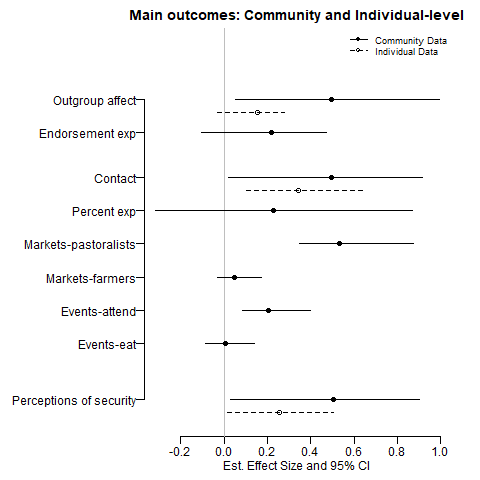
\includegraphics[width=\linewidth]{../../figs/ecpn_coefplots_MainOuts-cats.png}
        %\caption{Look at fig 1!}
        \label{fig:fig1}
    \end{minipage}
    \hfill
    \begin{minipage}[b]{.48\textwidth}
        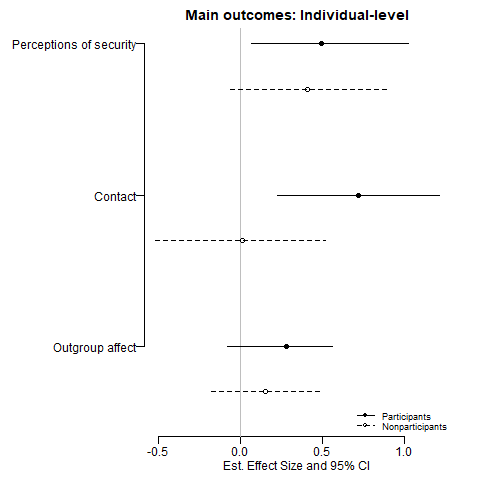
\includegraphics[width=\linewidth]{../../figs/ecpn_coefplots_MainOuts_panel-cats.png}
        %\caption{Look at fig 2!}
        \label{fig:fig2}
    \end{minipage}
\end{figure}

\hypertarget{intergroup-affect}{%
\subsection{Intergroup Affect}\label{intergroup-affect}}

ECPN bolstered intergroup affect in treatment communities. Respondents
in treatment communities report more trust the other group and are more
comfortable engaging in various relationships with the outgroup, such as
trading goods and intermarriage. Intergroup affect as measured by the
endorsement experiment also improves more in the treatment group than
the control group, though the difference is not statistically
significant at conventional levels.

Figures 3 and 4 show the effect of ECPN on the intergroup affect survey
index. Descriptively, affect in control communities decreased from
baseline to endline, while intervention communities improved over the
same time period. As measured by the endorsement experiment, affect
declines in both treatment and control communities, but declines more in
control communities. Both measures suggest that ECPN improved affect
towards the outgroup.

\begin{figure}[!h]
    \begin{minipage}[b]{.48\textwidth}
        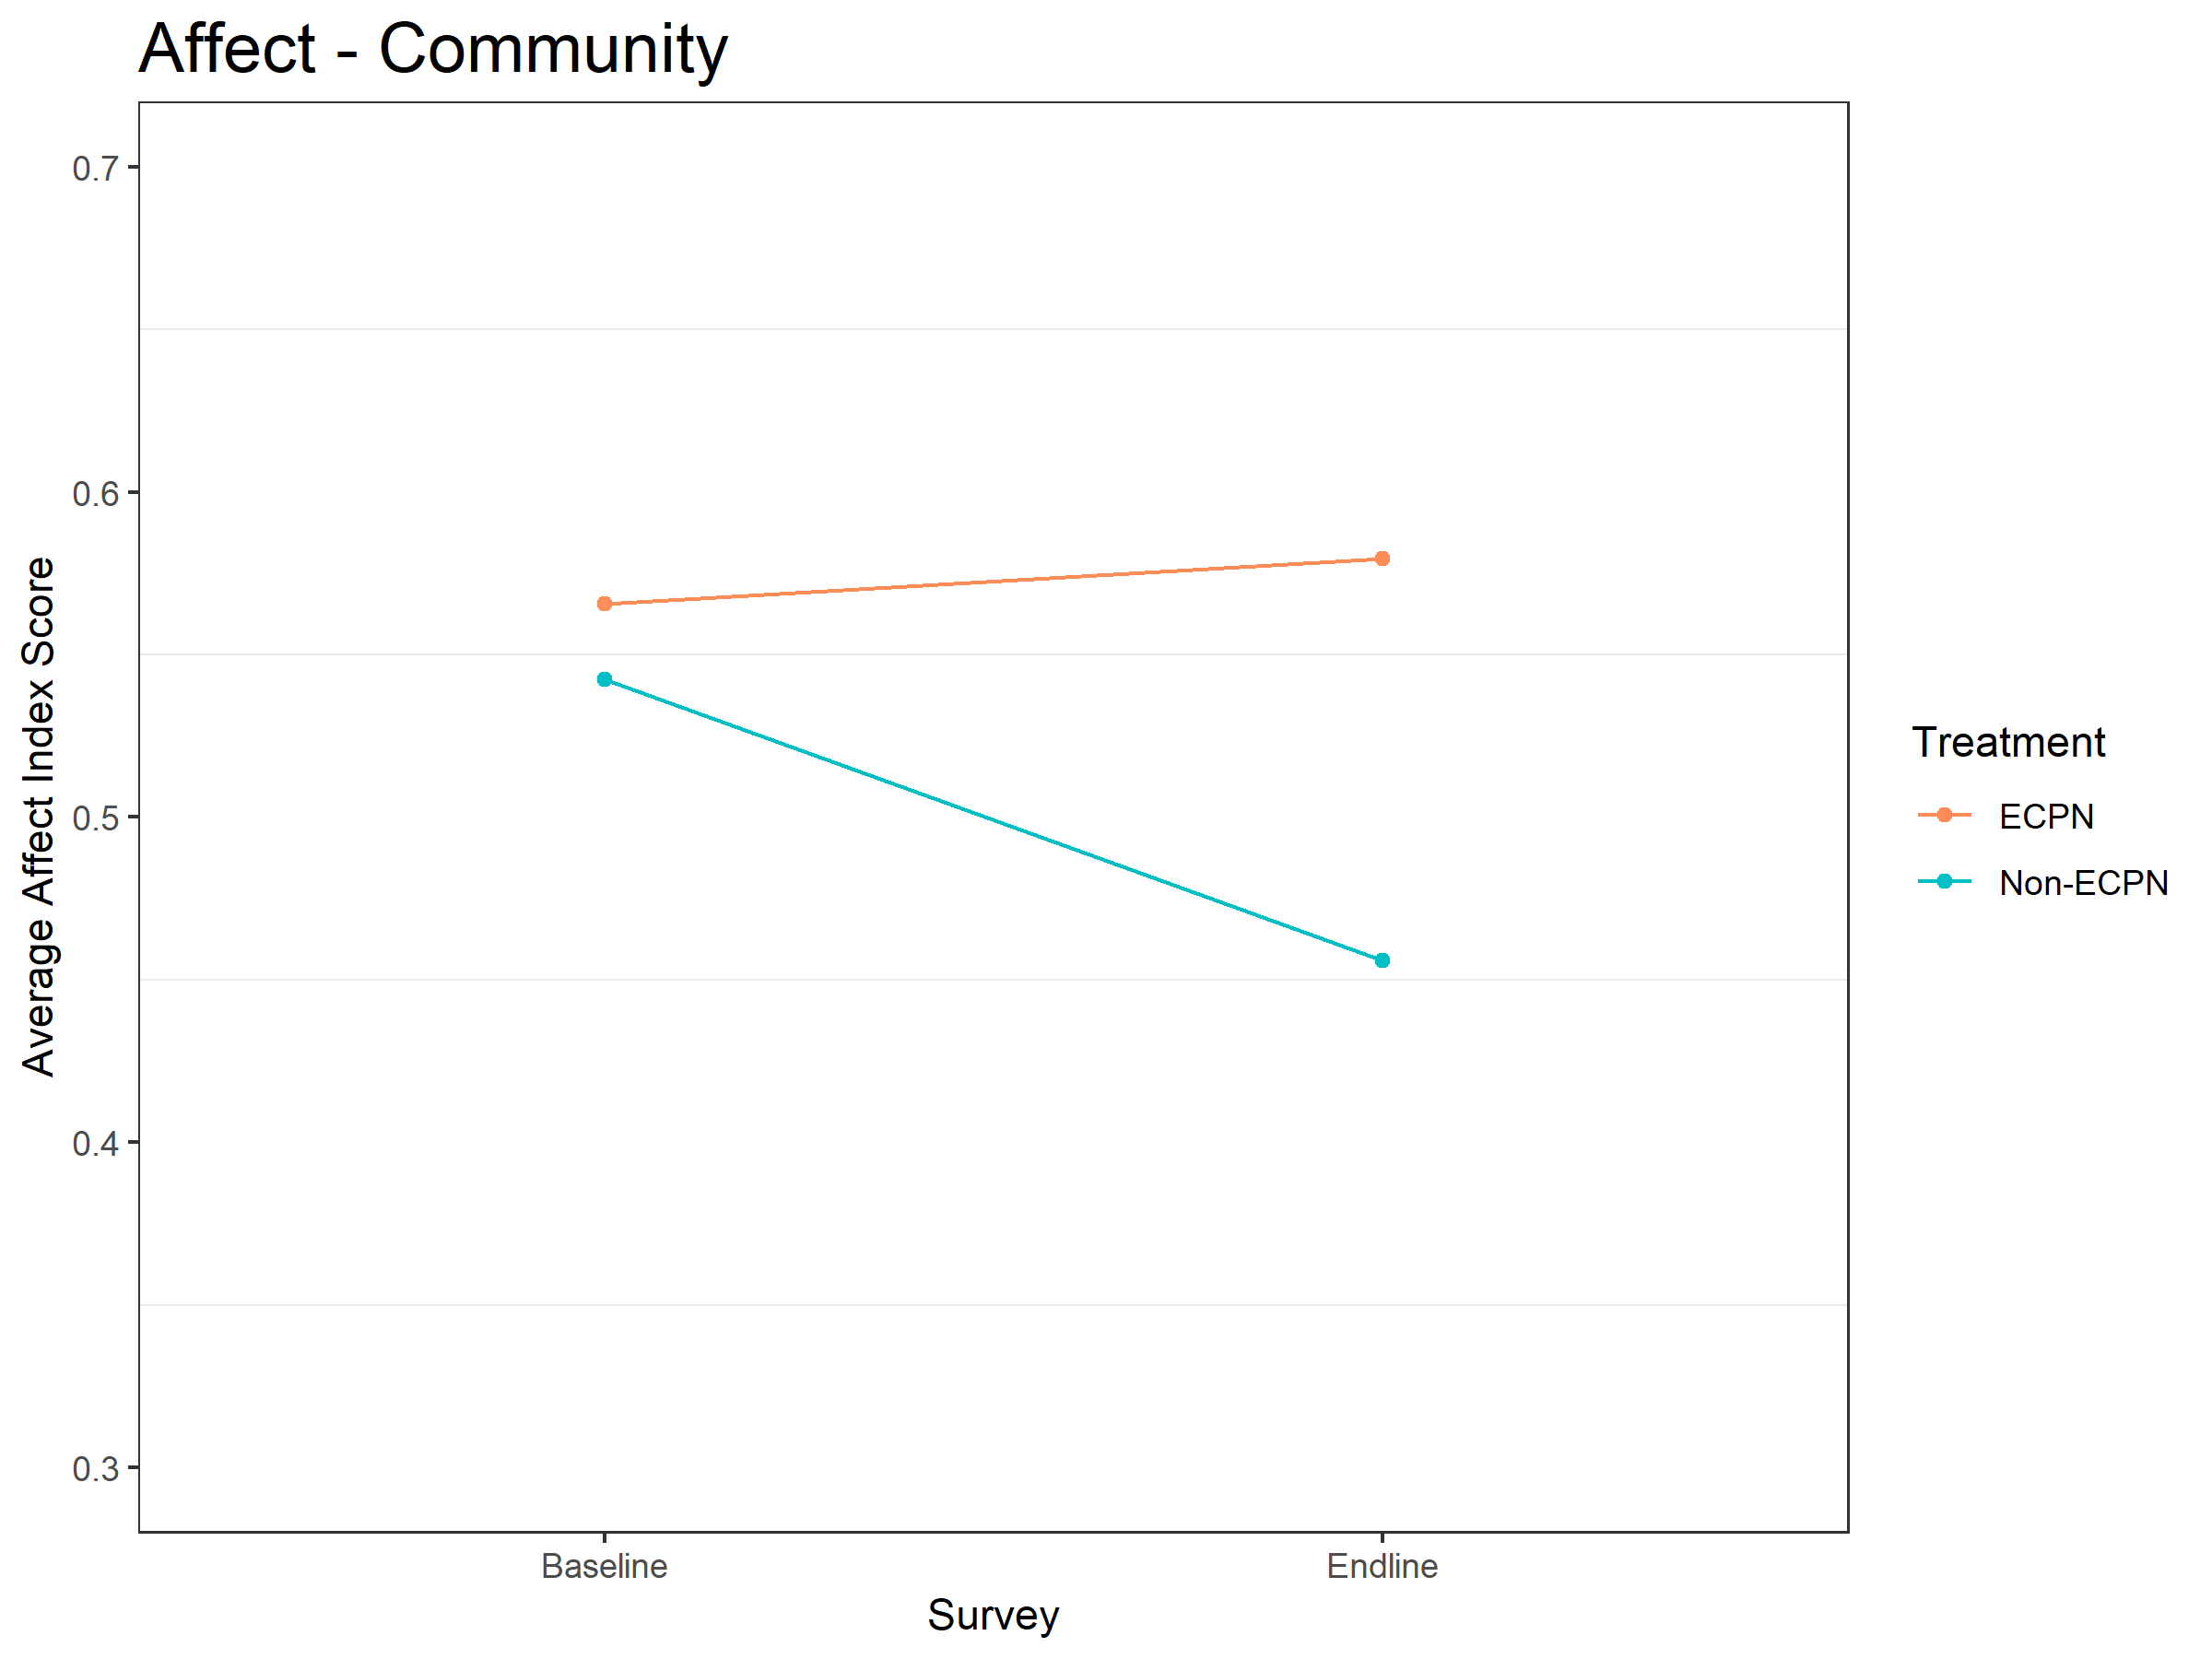
\includegraphics[width=\linewidth]{../../figs/affectComm_plot.png}
        %\caption{Look at fig 1!}
        \label{fig:fig3}
    \end{minipage}
    \hfill
    \begin{minipage}[b]{.48\textwidth}
        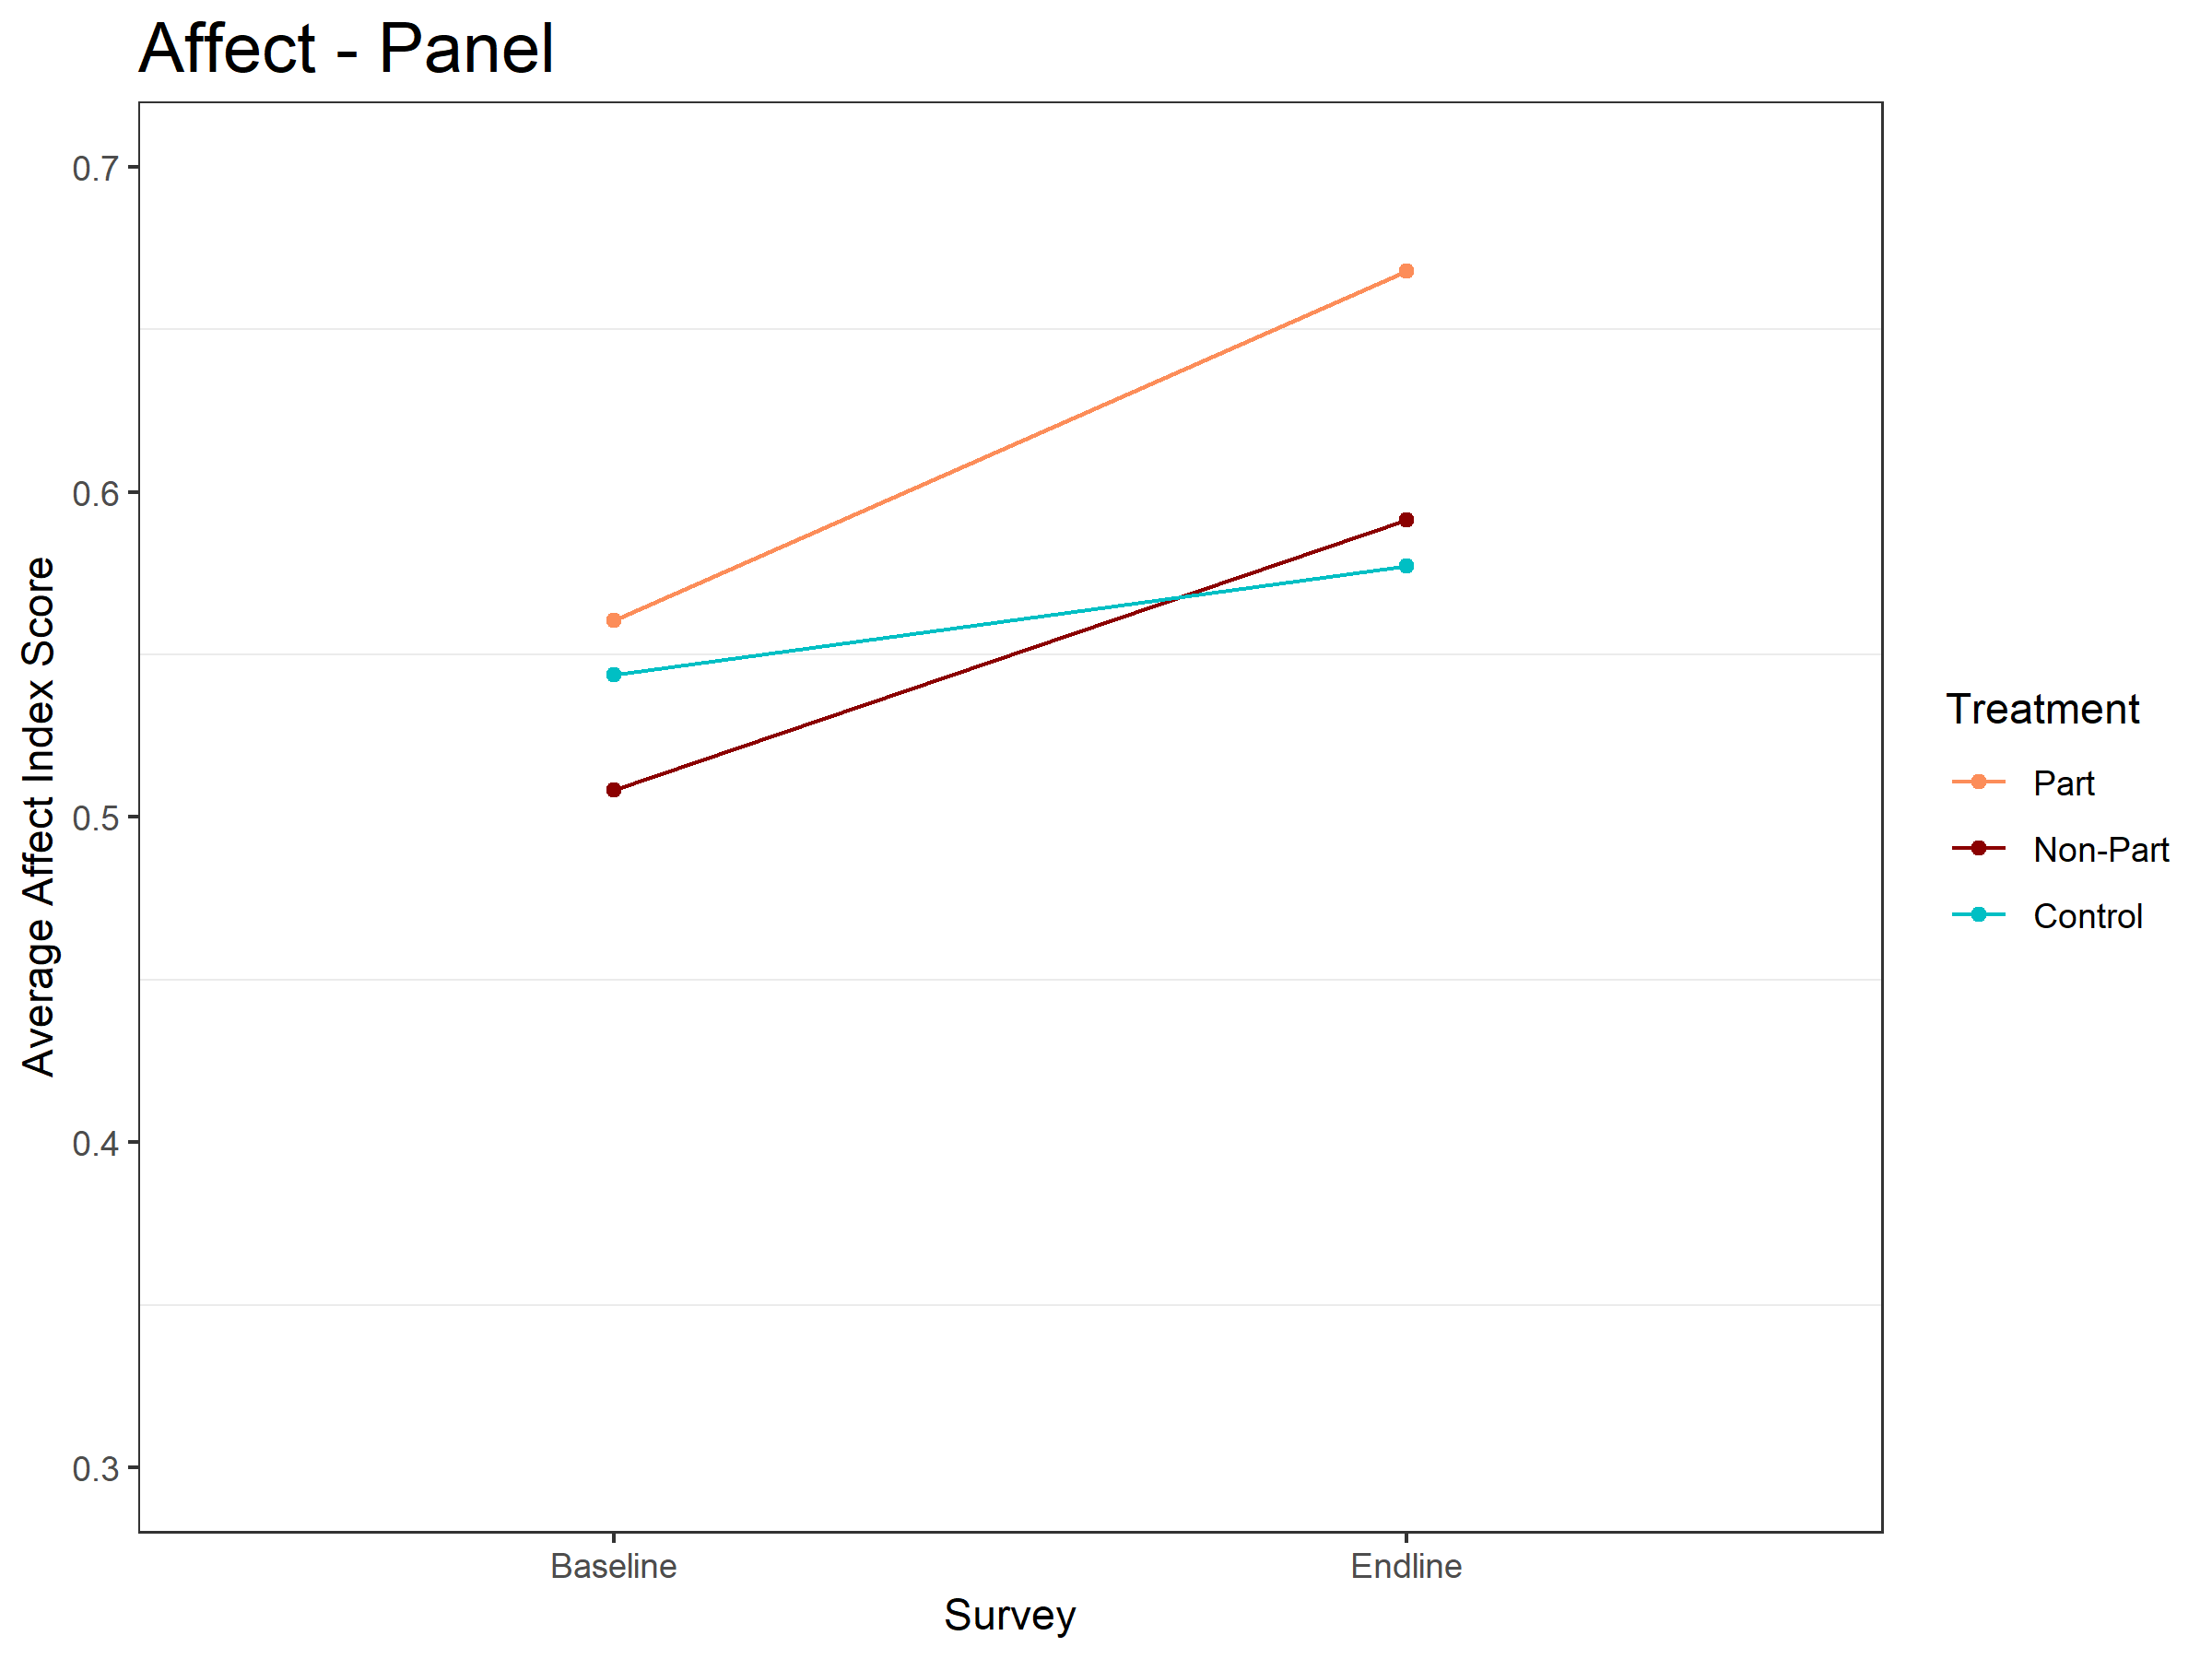
\includegraphics[width=\linewidth]{../../figs/affectPan_plot.png}
        %\caption{Look at fig 2!}
        \label{fig:fig4}
    \end{minipage}
\end{figure}

\hypertarget{contact}{%
\subsection{Contact}\label{contact}}

The effect of ECPN on contact is substantial. Respondents in treatment
communities report more contact and more willingness to engage in
contact at all levels of the percent experiment; we also observe more
pastoralists in markets interacting with farmers. Since the markets are
all located in the farming community, the sustained presence of
pastoralists there suggests that (1) farmers were accepting/tolerant of
pastoralists in their community and (2) pastoralists felt comfortable
spending time in the farmer community. The number of farmers present in
the markets does not change in either group, which makes sense because
the market is inside the farming community.

\begin{figure}[!h]
    \begin{minipage}[b]{.48\textwidth}
        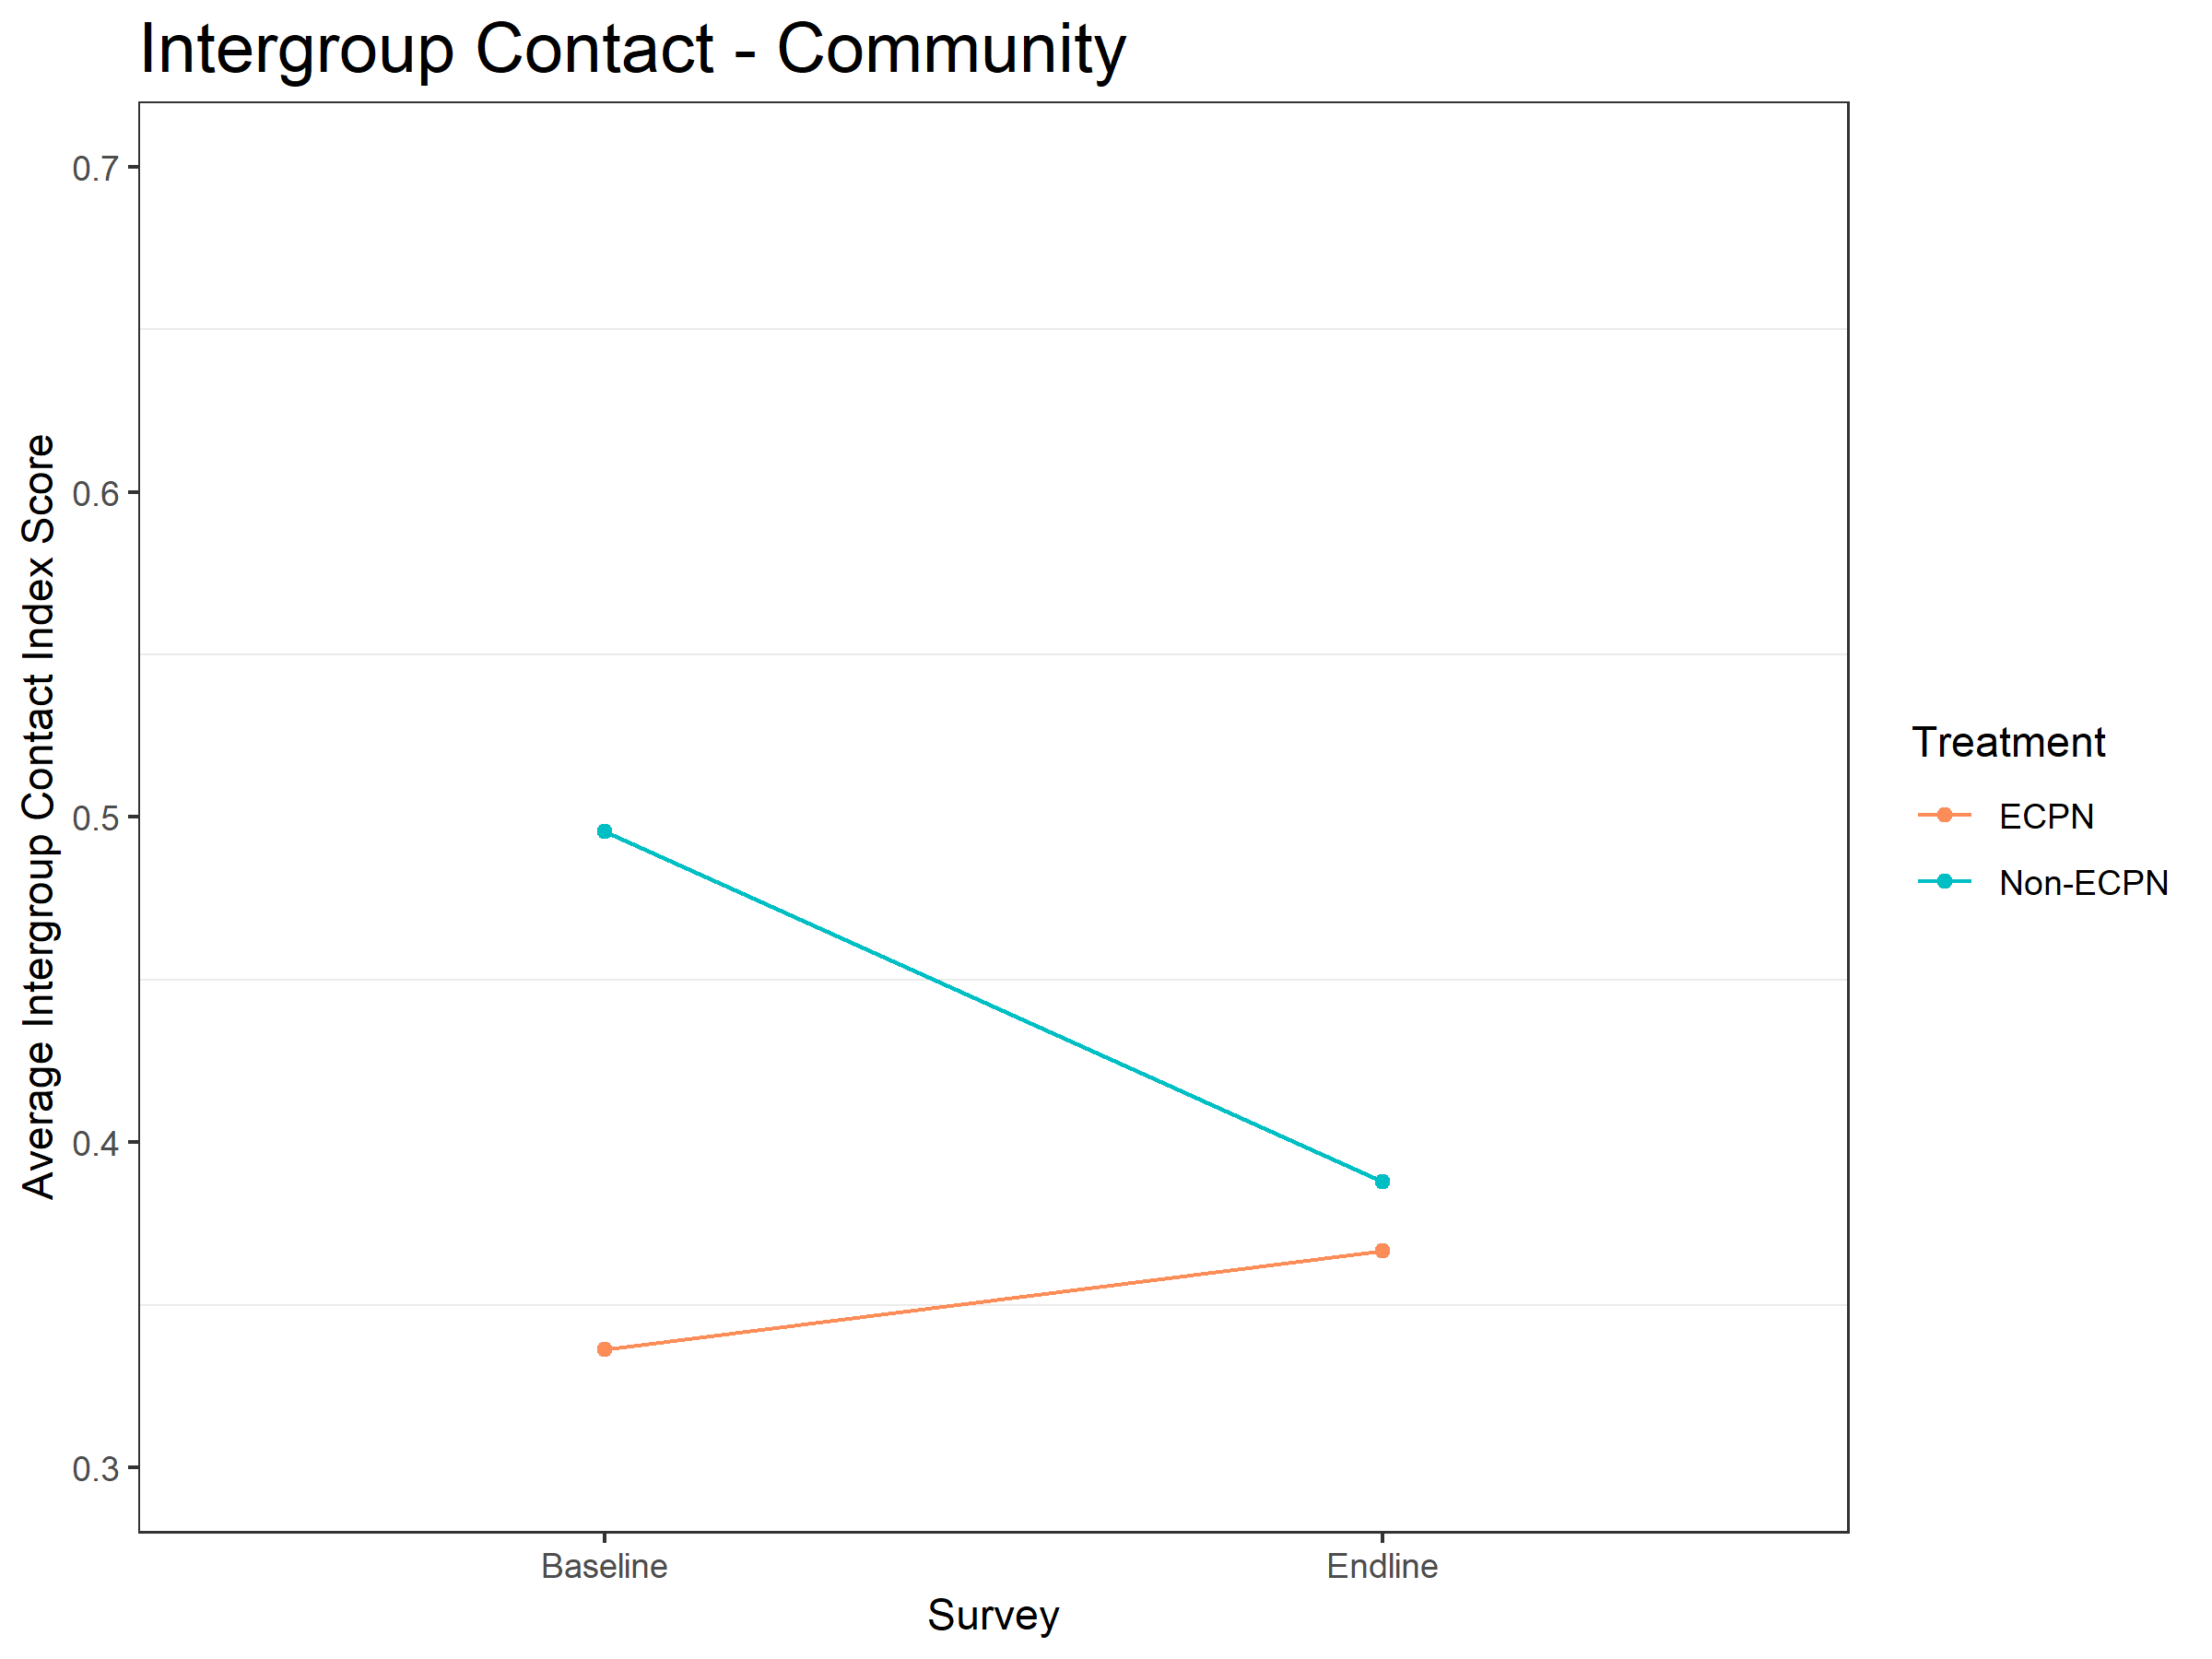
\includegraphics[width=\linewidth]{../../figs/conComm_plot.png}
        %\caption{Look at fig 1!}
        \label{fig:fig5}
    \end{minipage}
    \hfill
    \begin{minipage}[b]{.48\textwidth}
        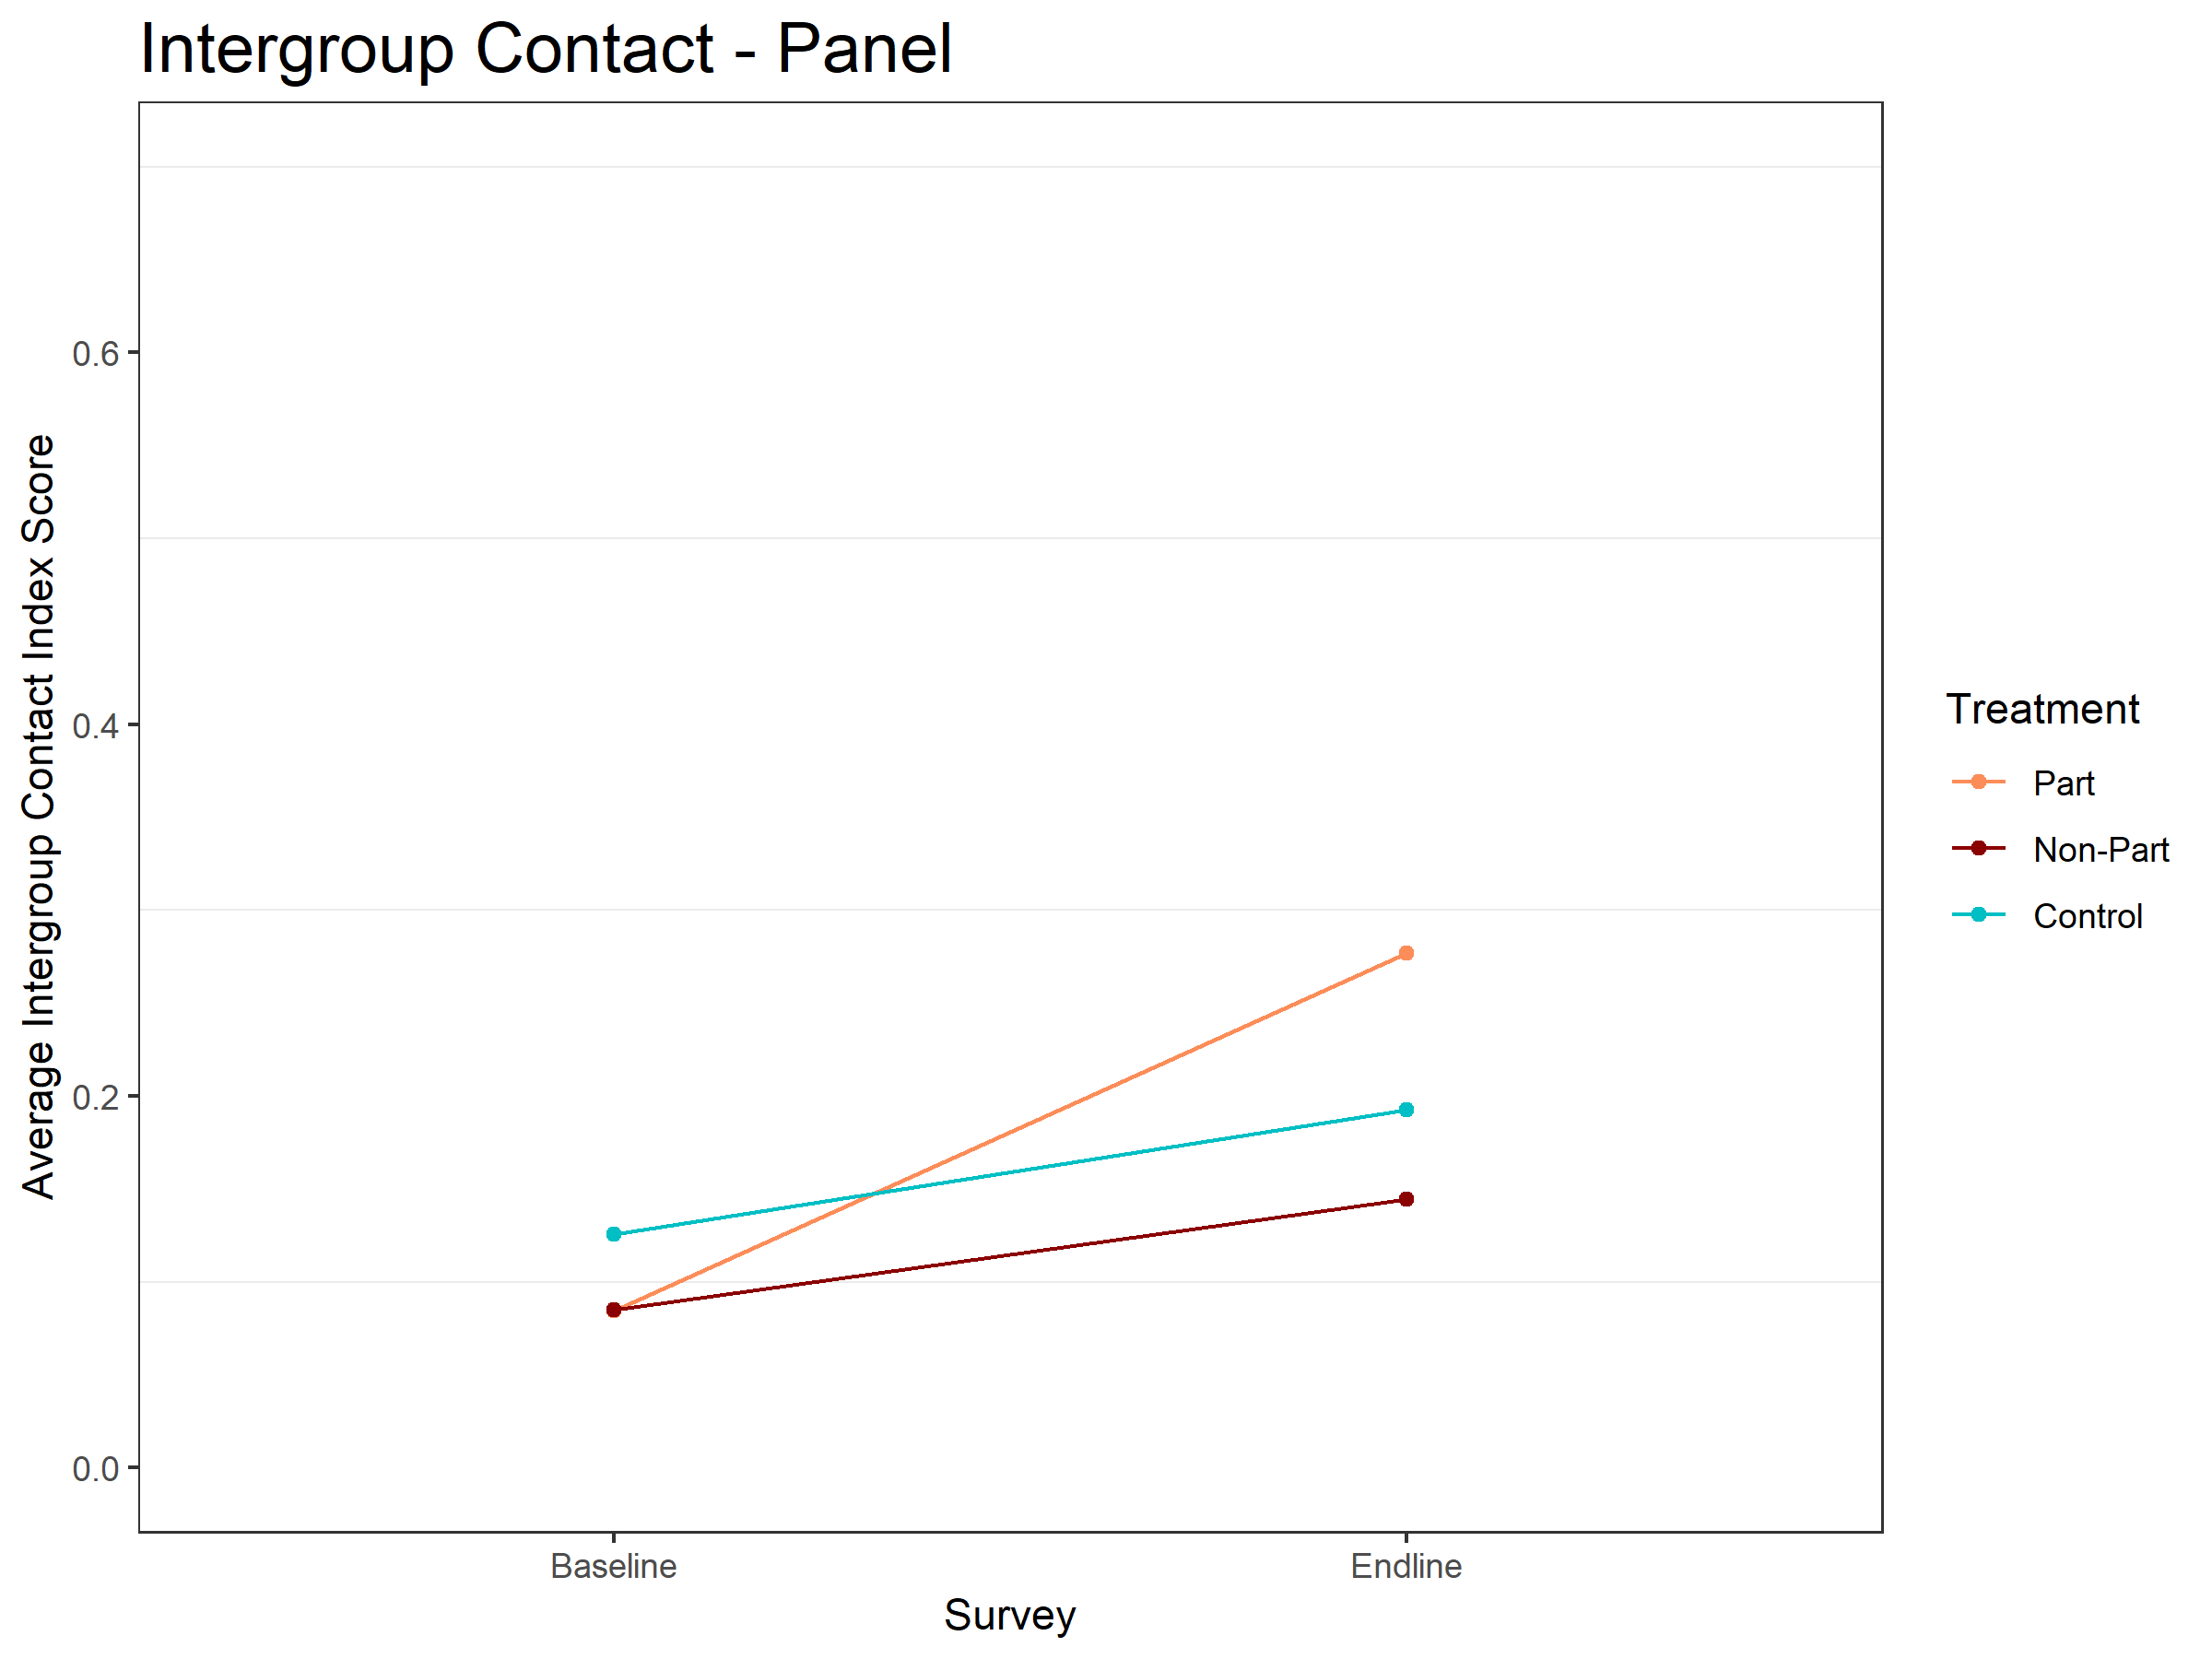
\includegraphics[width=\linewidth]{../../figs/conPan_plot.png}
        %\caption{Look at fig 2!}
        \label{fig:fig6}
    \end{minipage}
\end{figure}

Figures 5 and 6 shows the effect of ECPN on the contact survey outcomes.
Descriptively, the community-level self-reports show that intergroup
contact declined sharply in control communities but rose slightly in
treatment communities. It is impressive that ECPN increased contact
while the social environment led to a sharp decline in control sites.
The secular decline is due to the displacement in Benue, where
intergroup contact went down for every group, though it declined far
less in treatment sites. In Nasarawa, intergroup contact increased in
both treatment and control sites, but far more in treatment sites.

At the individual-level, intergroup contact increased for committee
participants but stayed largely the same for nonparticipants and
controls. The large community-level effect, however, suggests that the
effects of ECPN \emph{did} extend to nonparticipants in treatment
communities. But the effect did not extend to the type of nonparticipant
who we could track down and resurvey.

\hypertarget{insecurity}{%
\subsection{Insecurity}\label{insecurity}}

ECPN's substantially decreased feelings of insecurity in the treatment
group. The effect is large in both the community-level and the
individual-level data. Security in ECPN communities improved far more
from baseline to endline than in control communities. At the
individual-level, participants and nonparticipants improved equally,
suggesting that these increases reflect a change in the conflict
environment that impacts the entire community, not just respondents
involved in ECPN committees. These improvements in treatment communities
are especially powerful because other survey questions show that ECPN
increased awareness of the conflict -- respondents in ECPN communities
are more likely than the control to know that violence between groups
has occurred recently, yet they feel more secure.

\begin{figure}[!h]
    \begin{minipage}[b]{.48\textwidth}
        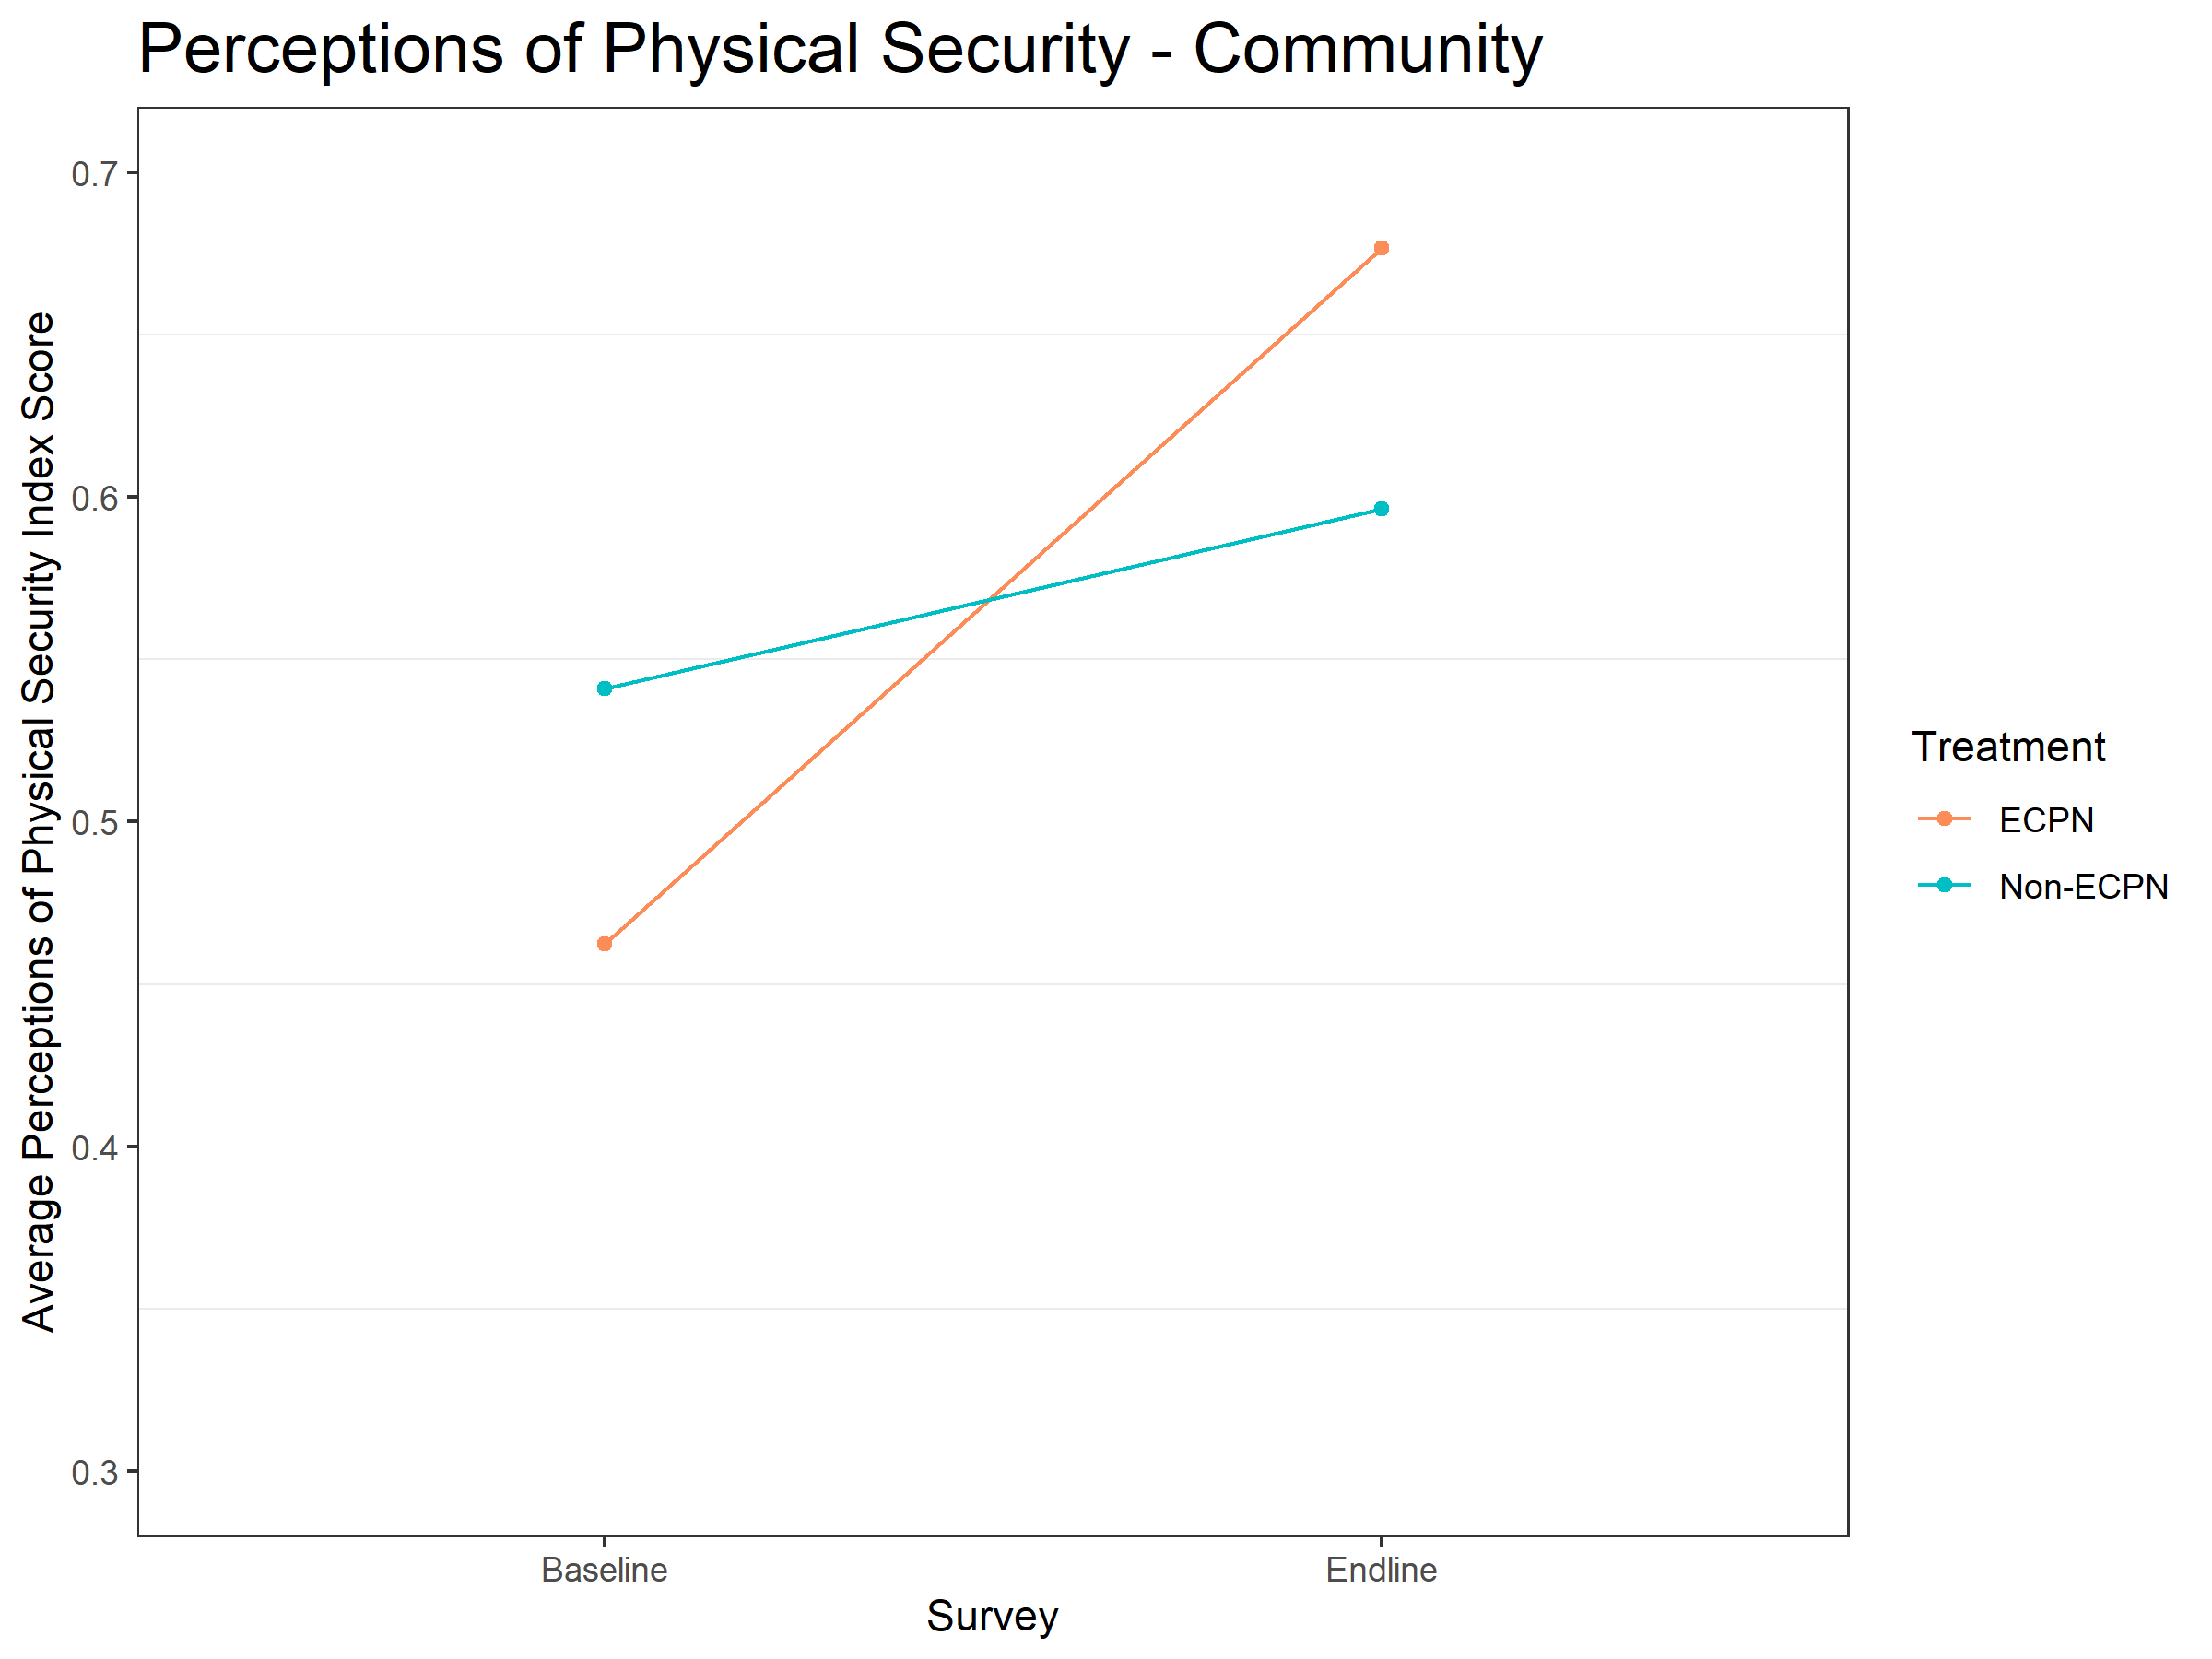
\includegraphics[width=\linewidth]{../../figs/inComm_plot.png}
        %\caption{Look at fig 1!}
        \label{fig:fig7}
    \end{minipage}
    \hfill
    \begin{minipage}[b]{.48\textwidth}
        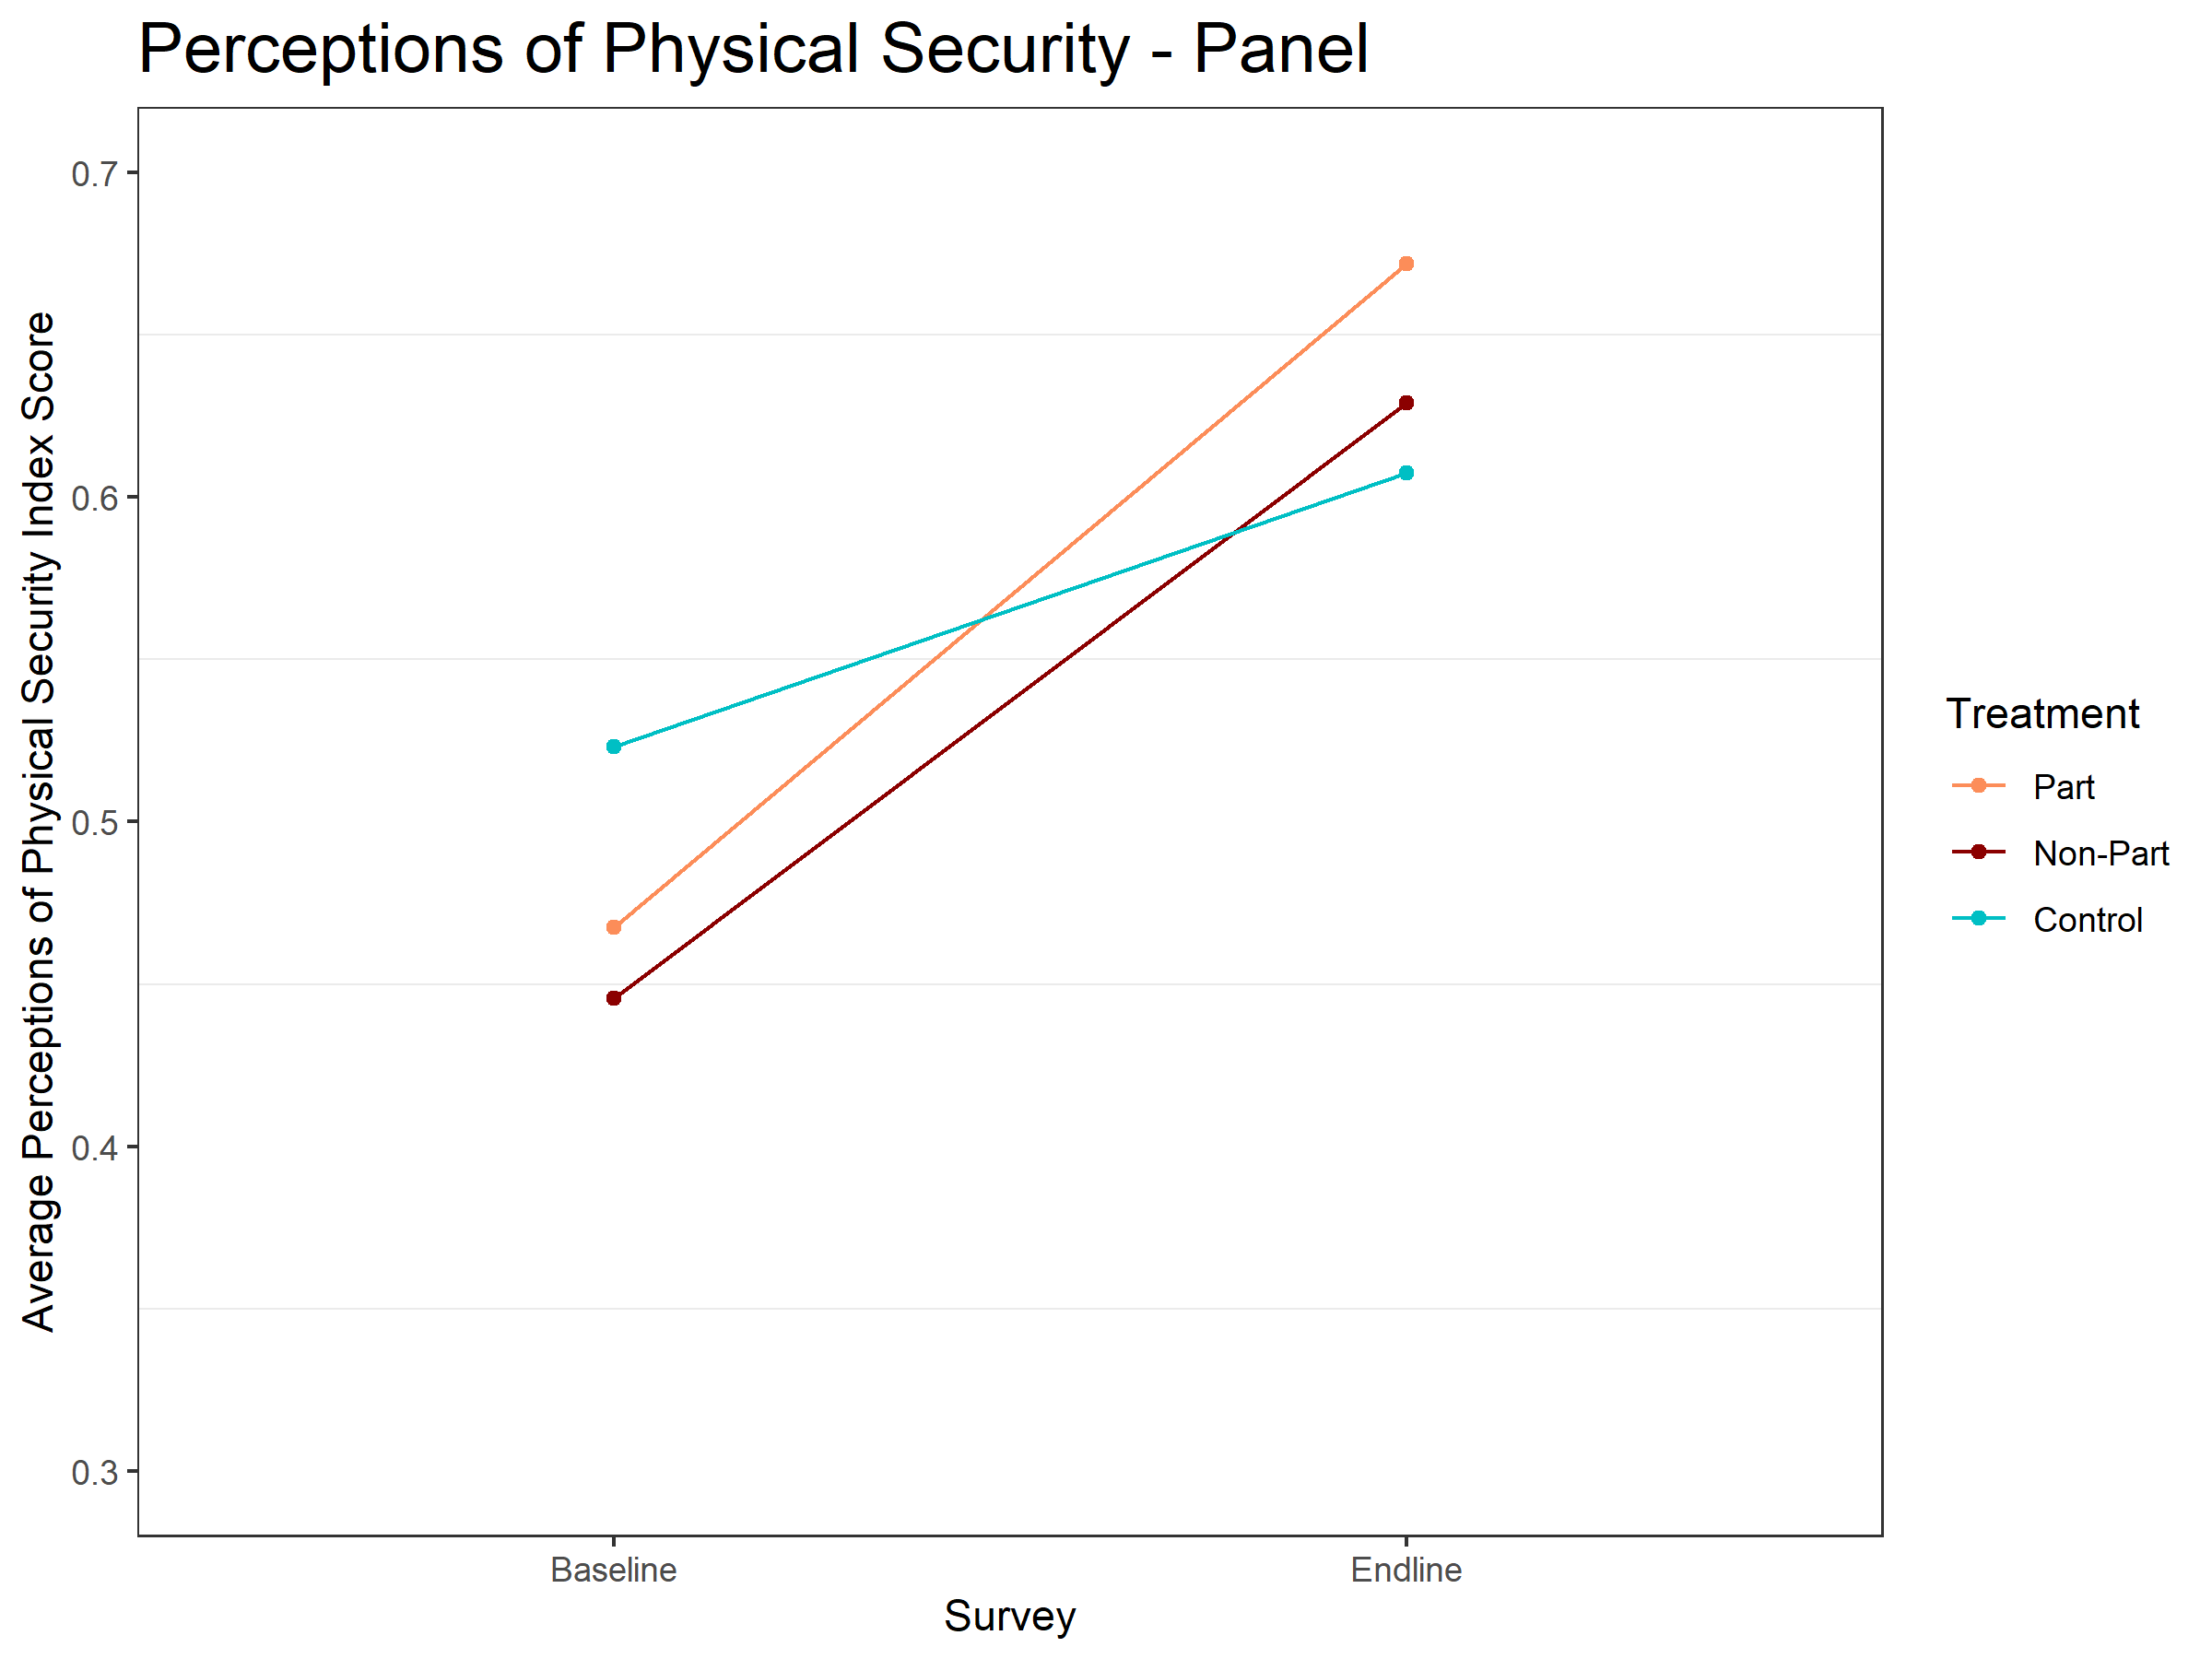
\includegraphics[width=\linewidth]{../../figs/inPan_plot.png}
        %\caption{Look at fig 2!}
        \label{fig:fig8}
    \end{minipage}
\end{figure}

Figures 7 and 8 show the effect of ECPN on insecurity. Descriptively,
the insecurity of control communities is largely unchanged from baseline
to endline but insecurity in treatment communities declines
substantially. ECPN communities initially felt more insecure than
control communities but were more secure at the end of the program. ECPN
substantially the security of people in intervention communities.

\hypertarget{placebo-attitudes-about-violence}{%
\subsection{Placebo: attitudes about
violence}\label{placebo-attitudes-about-violence}}

To provide evidence that these survey results are due to intergroup
contact and not due to social desirability bias, we analyze the effect
of ECPN on attitudes about violence. If ECPN affects attitudes about
violence, then we worry that other self-reports were affected by social
desirability bias. If ECPN has no effect on attitudes about violence,
then it is unlikely that other self-reports were affected by social
desirability bias.

ECPN has no effect on attitudes about violence in the community-level
data or the individual-level data. {[}note: will add table{]} Table 1
shows two different ways of estimating the effect and two different ways
of measuring attitudes about violence.

\hypertarget{mechanisms-empathy-threat-and-ingroup-expansion}{%
\subsection{Mechanisms: Empathy, Threat, and Ingroup
Expansion}\label{mechanisms-empathy-threat-and-ingroup-expansion}}

Our results suggest that ECPN improved intergroup relations between
farmers and pastoralists. We also undertook an exploratory analysis to
learn the mechanisms through which ECPN affected attitudes. Based on the
literature about contact theory, we looked for evidence that ECPN worked
through empathy and perspective-taking, reduced feelings of threat, and
expansion of the respondent's ingroup to include the former outgroup.

Our exploratory analysis suggests that ECPN may have worked through
increasing empathy. ECPN led to increased empathy in the community and
individual-level analyses. In turn, increased empathy correlated with
improved intergroup affect in the community-level data and with
increases in intergroup affect and intergroup contact at the individual
level. Increased perspective-taking also correlated with intergroup
affect and intergroup contact in both analyses. ECPN may have led to
increased perspective-taking, though not quite to a statistically
significant level. Though this analysis is only exploratory, it suggests
that increased empathy is a plausible mechanism through which ECPN
improved intergroup relations. Because empathy was not randomly
assigned, though, it's equally plausible that ECPN improved intergroup
affect and fostered intergroup contact, and that those outcomes led to
increased empathy.

There is no evidence that ECPN reduced perceptions of threat or expanded
perceptions of the ingroup. ECPN did not effect either survey index, and
the public goods game shows that the treatment group was not better at
coordinating than the control group. Treatment communities donated
\emph{less} to the shared community fund than control communities. At
the individual-level, ECPN participants donated less than
nonparticipants who donated less than respondents in the control group.
This is the opposite pattern of what we would expect if intergroup
contact caused the communities to think of each other as part of one
ingroup. Reduced threat and ingroup expansion are still plausible
psychological mechanisms -- each correlated strongly with at least one
outcome -- though neither was increased by ECPN.

{[}Table: Rows are mechanisms, columns are outcomes, separated by
community vs individual analyses. Show coefficient (pvalue).{]}

\hypertarget{discussion}{%
\section{Discussion}\label{discussion}}

This paper provides evidence that intergroup contact can improve
intergroup relations, even in dire circumstances. We tested a
programmatic contact intervention in an active and escalating conflict
between farmers and pastoralists in Nigeria. This context poses a tough
test for contact to improve intergroup relations because the groups'
material, social, and psychological incentives are opposed. Despite the
difficult context, the program improved intergroup affect, fostered more
intergroup contact, and decreased feelings of insecurity in these
communities. Methodologically, this study highlights the benefits of
measuring outcomes at baseline and endline in a treatment group and in a
control group as a means of capturing the secular trend.

We join a number of studies testing the effects of contact in real-world
conflict situations. More studies need to be conducted to determine the
limits of contact and the conditions under which contact can effectively
improve intergroup relations. In our case, we believe that the presence
of a shared latent interest was the condition necessary for contact to
improve relations and improve prospects for peace. Cooperative contact
helps reveal the latent shared interest to both groups by demonstrating
how the groups can work together to achieve a common goal and removing
psychological and social barriers to identifying the shared interest.
Contact also provides the groups with opportunities to send costly
signals of their intent to cooperate, which are important for intergroup
cooperation (Kydd 2000).

This study highlights several opportunities to learn about the effects
of contact in conflict environments. First, since our goal was to test
the hypothesis that contact would improve group relations in an active
conflict, we did not attempt to bring causal evidence to the question of
\emph{how} contact improves group relations. Our analysis of mechanisms
was only exploratory but suggests that contact may have worked through
increased empathy. Second, our program was implemented and randomized at
the community-level, not at the individual-level. Future studies should
consider how much contact it takes to improve attitudes, as well as how
social norms and interpersonal discussion diffuse the positive effects
of contact to individuals without outgroup contact.

Third, contact interventions, explicitly or implicitly, involve the
groups cooperating to \emph{achieve} a joint goal. But what if contact
is not successful and the goal is not achieved? Does contact itself
still improve attitudes, or does contact work because groups begin to
associate cross-group cooperation with good outcomes? In a similar vein,
are Allport's conditions necessary for contact to achieve its aims, or
are they only needed insofar as they ensure the intergroup cooperation
generates positive outcomes for both groups?

Lastly, we see an opportunity for collaboration between scholars of
intergroup contact and scholars of conflict. These literatures are often
concerned with the same end goals -- reducing conflict -- but rarely
speak to one another. Conflict scholars often see conflict as a
bargaining problem, and violence as a bargaining failure. This
literature points to a lack of trust as the primary cause of conflict
and usually posit a strong third party actor as necessary to guarantee
peace. Intergroup contact research hints that intergroup contact can
create cooperative norms that serve the same function as a strong third
party, perhaps by encouraging ingroup policing (Fearon and Laitin 1996).
Improving relations -- especially improving trust -- through
psychological interventions like intergroup contact can help groups
overcome commitment problems and reduce the likelihood of violence.

\hypertarget{references}{%
\section*{References}\label{references}}
\addcontentsline{toc}{section}{References}

\hypertarget{refs}{}
\leavevmode\hypertarget{ref-nyt2018nigeria}{}%
Akinwotu, Emmanuel. 2018. ``Nigeria's Farmers and Herders Fight a Deadly
Battle for Scarce Resources.'' \emph{New York Times}.
\url{https://www.nytimes.com/2018/06/25/world/africa/nigeria-herders-farmers.html}.

\leavevmode\hypertarget{ref-allport1954prejudice}{}%
Allport, Gordon. 1954. ``The Nature of Prejudice.'' \emph{Garden City,
NJ Anchor}.

\leavevmode\hypertarget{ref-al2013intergroup}{}%
Al Ramiah, Ananthi, and Miles Hewstone. 2013. ``Intergroup Contact as a
Tool for Reducing, Resolving, and Preventing Intergroup Conflict:
Evidence, Limitations, and Potential.'' \emph{American Psychologist}
68(7): 527.

\leavevmode\hypertarget{ref-barnhardt2009near}{}%
Barnhardt, Sharon. 2009. ``Near and Dear? Evaluating the Impact of
Neighbor Diversity on Inter-Religious Attitudes.'' \emph{Unpublished
working paper}.

\leavevmode\hypertarget{ref-bar2000intractable}{}%
Bar-Tal, Daniel. 2000. ``From Intractable Conflict Through Conflict
Resolution to Reconciliation: Psychological Analysis.'' \emph{Political
Psychology} 21(2): 351--65.

\leavevmode\hypertarget{ref-bar2017development}{}%
Bar-Tal, Daniel, and Talia Avrahamzon. 2017. ``Development of
Delegitimization and Animosity in the Context of Intractable Conflict.''

\leavevmode\hypertarget{ref-bassett2009mobile}{}%
Bassett, Thomas J. 2009. ``Mobile Pastoralism on the Brink of Land
Privatization in Northern côte d'Ivoire.'' \emph{Geoforum} 40(5):
756--66.

\leavevmode\hypertarget{ref-batson1997empathy}{}%
Batson, C Daniel et al. 1997. ``Empathy and Attitudes: Can Feeling for a
Member of a Stigmatized Group Improve Feelings Toward the Group?''
\emph{Journal of personality and social psychology} 72(1): 105.

\leavevmode\hypertarget{ref-broockman2016durably}{}%
Broockman, David, and Joshua Kalla. 2016. ``Durably Reducing
Transphobia: A Field Experiment on Door-to-Door Canvassing.''
\emph{Science} 352(6282): 220--24.

\leavevmode\hypertarget{ref-burns2015interaction}{}%
Burns, Justine, Lucia Corno, and Eliana La Ferrara. 2015.
\emph{Interaction, Prejudice and Performance. Evidence from South
Africa}. Working paper.

\leavevmode\hypertarget{ref-carrell2015impact}{}%
Carrell, Scott E, Mark Hoekstra, and James E West. 2015. \emph{The
Impact of Intergroup Contact on Racial Attitudes and Revealed
Preferences}. National Bureau of Economic Research.

\leavevmode\hypertarget{ref-christ2014contextual}{}%
Christ, Oliver et al. 2014. ``Contextual Effect of Positive Intergroup
Contact on Outgroup Prejudice.'' \emph{Proceedings of the National
Academy of Sciences} 111(11): 3996--4000.

\leavevmode\hypertarget{ref-cook1985experimenting}{}%
Cook, Stuart W. 1985. ``Experimenting on Social Issues: The Case of
School Desegregation.'' \emph{American Psychologist} 40(4): 452.

\leavevmode\hypertarget{ref-cook1971race}{}%
Cook, Stuart Wellford, Lawrence Samuel Wrightsman, and Shirley
Wrightsman. 1971. \emph{The Effect of Unintended Interracial Contact
Upon Racial Interaction and Attitude Change}. Educational resources in
information center, US Department of health, education \& welfare.

\leavevmode\hypertarget{ref-cotula2004land}{}%
Cotula, Lorenzo, Camilla Toulmin, Ced Hesse, and others. 2004.
\emph{Land Tenure and Administration in Africa: Lessons of Experience
and Emerging Issues}. International Institute for Environment;
Development London.

\leavevmode\hypertarget{ref-daniel2018anti}{}%
Daniel, Soni. 2018. ``Anti-Open Grazing Law: Nass, Benue, Kwara, Taraba
Tackle Defence Minister.'' \emph{Vanguard}.
\url{https://www.vanguardngr.com/2018/06/anti-open-grazing-law-nass-benue-kwara-taraba-tackle-defence-minister/}.

\leavevmode\hypertarget{ref-deutsch1973resolution}{}%
Deutsch, Morton. 1973. \emph{The Resolution of Conflict: Constructive
and Destructive Processes}. Yale University Press.

\leavevmode\hypertarget{ref-deutsch1951interracial}{}%
Deutsch, Morton, and Mary Evans Collins. 1951. \emph{Interracial
Housing: A Psychological Evaluation of a Social Experiment}. U of
Minnesota Press.

\leavevmode\hypertarget{ref-ditlmann2016can}{}%
Ditlmann, Ruth K, and Cyrus Samii. 2016. ``Can Intergroup Contact Affect
Ingroup Dynamics? Insights from a Field Study with Jewish and
Arab-Palestinian Youth in Israel.'' \emph{Peace and Conflict: Journal of
Peace Psychology} 22(4): 380.

\leavevmode\hypertarget{ref-ditlmann2017addressing}{}%
Ditlmann, Ruth K, Cyrus Samii, and Thomas Zeitzoff. 2017. ``Addressing
Violent Intergroup Conflict from the Bottom up?'' \emph{Social Issues
and Policy Review} 11(1): 38--77.

\leavevmode\hypertarget{ref-doosje1995bad}{}%
Doosje, Bertjan, Russell Spears, and Willem Koomen. 1995. ``When Bad
Isn't All Bad: Strategic Use of Sample Information in Generalization and
Stereotyping.'' \emph{Journal of Personality and Social psychology}
69(4): 642.

\leavevmode\hypertarget{ref-dovidio2017reducing}{}%
Dovidio, John F, Angelika Love, Fabian MH Schellhaas, and Miles
Hewstone. 2017. ``Reducing Intergroup Bias Through Intergroup Contact:
Twenty Years of Progress and Future Directions.'' \emph{Group Processes
\& Intergroup Relations} 20(5): 606--20.

\leavevmode\hypertarget{ref-duncan1976differential}{}%
Duncan, Birt L. 1976. ``Differential Social Perception and Attribution
of Intergroup Violence: Testing the Lower Limits of Stereotyping of
Blacks.'' \emph{Journal of personality and social psychology} 34(4):
590.

\leavevmode\hypertarget{ref-duru2018court}{}%
Duru, Peter. 2018. ``Court Stops Inspector General from Proscribing
Benue Livestock Guard.'' \emph{Vanguard}.
\url{https://www.vanguardngr.com/2018/11/court-stops-ig-from-proscribing-benue-livestock-guards/}.

\leavevmode\hypertarget{ref-economist2019militias}{}%
Economist, The. 2019. ``Malicious Malitias: States in the Sahel Have
Unleashed Ethnic Gangs with Guns.'' \emph{The Economist}.
\url{https://www.economist.com/middle-east-and-africa/2019/05/04/states-in-the-sahel-have-unleashed-ethnic-gangs-with-guns}.

\leavevmode\hypertarget{ref-fulanisize2017}{}%
Encyclopedia, New World. 2017. ``Fulani --- New World Encyclopedia,''
\url{//www.newworldencyclopedia.org/p/index.php?title=Fulani\&oldid=1004777}.

\leavevmode\hypertarget{ref-fearon1995rationalist}{}%
Fearon, James D. 1995. ``Rationalist Explanations for War.''
\emph{International organization} 49(3): 379--414.

\leavevmode\hypertarget{ref-fearon1996explaining}{}%
Fearon, James D, and David D Laitin. 1996. ``Explaining Interethnic
Cooperation.'' \emph{American political science review} 90(4): 715--35.

\leavevmode\hypertarget{ref-fearon2000violence}{}%
---------. 2000. ``Violence and the Social Construction of Ethnic
Identity.'' \emph{International organization} 54(4): 845--77.

\leavevmode\hypertarget{ref-festinger1962cognitiveDissonance}{}%
Festinger, Leon. 1962. 2 \emph{A Theory of Cognitive Dissonance}.
Stanford university press.

\leavevmode\hypertarget{ref-forbes1997ethnic}{}%
Forbes, Hugh Donald. 1997. \emph{Ethnic Conflict: Commerce, Culture, and
the Contact Hypothesis}. Yale University Press.

\leavevmode\hypertarget{ref-gaertner2014reducing}{}%
Gaertner, Samuel L, and John F Dovidio. 2014. \emph{Reducing Intergroup
Bias: The Common Ingroup Identity Model}. Psychology Press.

\leavevmode\hypertarget{ref-gaertner1993common}{}%
Gaertner, Samuel L et al. 1993. ``The Common Ingroup Identity Model:
Recategorization and the Reduction of Intergroup Bias.'' \emph{European
review of social psychology} 4(1): 1--26.

\leavevmode\hypertarget{ref-gubler2013humanizing}{}%
Gubler, Joshua R. 2013. ``When Humanizing the Enemy Fails: The Role of
Dissonance and Justification in Intergroup Conflict.'' In \emph{Annual
Meeting of the American Political Science Association},

\leavevmode\hypertarget{ref-frontera2018nigeria}{}%
Hailemariam, Adium. 2018. ``Nigeria: Violence in the Middle Belt Becomes
Major Concern for President Buhari.'' \emph{Frontera}.
\url{https://frontera.net/news/africa/nigeria-violence-in-the-middle-belt-becomes-major-concern-for-president-buhari/}.

\leavevmode\hypertarget{ref-council2019nigeria}{}%
Harwood, Asch. 2019. ``Update: The Numbers Behind Sectarian Violence in
Nigeria.'' \emph{Council on Foreign Relations}.
\url{https://www.cfr.org/blog/update-numbers-behind-sectarian-violence-nigeria}.

\leavevmode\hypertarget{ref-haslam2014dehumanization}{}%
Haslam, Nick, and Steve Loughnan. 2014. ``Dehumanization and
Infrahumanization.'' \emph{Annual review of psychology} 65: 399--423.

\leavevmode\hypertarget{ref-hewstone1996contact}{}%
Hewstone, Miles. 1996. ``Contact and Categorization: Social
Psychological.'' \emph{Stereotypes and stereotyping} 323.

\leavevmode\hypertarget{ref-fa2019deadly}{}%
Ilo, Udo Jude, Jonathan-Ichavar Ier, and Yemi Adamolekun. 2019. ``The
Deadliest Conflict You've Never Heard of: Nigeria's Cattle Herders and
Farmers Wage a Resource War.'' \emph{Foreign Affairs}.
\url{https://www.foreignaffairs.com/articles/nigeria/2019-01-23/deadliest-conflict-youve-never-heard}.

\leavevmode\hypertarget{ref-kertzer2018empathy}{}%
Kertzer, Joshua D, Ryan Brutger, and Kai Quek. 2018. ``Strategic Empathy
and the Security Dilemma: Cross-National Experimental Evidence from
China and the United States.''

\leavevmode\hypertarget{ref-klein1992motivated}{}%
Klein, William M, and Ziva Kunda. 1992. ``Motivated Person Perception:
Constructing Justifications for Desired Beliefs.'' \emph{Journal of
experimental social psychology} 28(2): 145--68.

\leavevmode\hypertarget{ref-kunda1990motivatedReasoning}{}%
Kunda, Ziva. 1990. ``The Case for Motivated Reasoning.''
\emph{Psychological bulletin} 108(3): 480.

\leavevmode\hypertarget{ref-kuusaana2015land}{}%
Kuusaana, Elias Danyi, and Kaderi Noagah Bukari. 2015. ``Land Conflicts
Between Smallholders and Fulani Pastoralists in Ghana: Evidence from the
Asante Akim North District (Aand).'' \emph{Journal of rural studies} 42:
52--62.

\leavevmode\hypertarget{ref-kydd2000trust}{}%
Kydd, Andrew. 2000. ``Trust, Reassurance, and Cooperation.''
\emph{International Organization} 54(2): 325--57.

\leavevmode\hypertarget{ref-lemmer2015can}{}%
Lemmer, Gunnar, and Ulrich Wagner. 2015. ``Can We Really Reduce Ethnic
Prejudice Outside the Lab? A Meta-Analysis of Direct and Indirect
Contact Interventions.'' \emph{European Journal of Social Psychology}
45(2): 152--68.

\leavevmode\hypertarget{ref-marmaros2006friendships}{}%
Marmaros, David, and Bruce Sacerdote. 2006. ``How Do Friendships Form?''
\emph{The Quarterly Journal of Economics} 121(1): 79--119.

\leavevmode\hypertarget{ref-mcdonnel2017graze}{}%
McDonnel, Tim. 2017. ``Why It's Now a Crime to Let Cattle Graze Freely
in 2 Nigerian States.'' \emph{National Public Radio (NPR)}.
\url{https://www.npr.org/sections/goatsandsoda/2017/12/12/569913821/why-its-now-a-crime-to-let-cattle-graze-freely-in-2-nigerian-states}.

\leavevmode\hypertarget{ref-mcdougal2015effect}{}%
McDougal, Topher L et al. 2015. ``The Effect of Farmer-Pastoralist
Violence on Income: New Survey Evidence from Nigeria's Middle Belt
States.'' \emph{Economics of Peace and Security Journal} 10(1): 54--65.

\leavevmode\hypertarget{ref-mousa2018overcome}{}%
Mousa, Salma. 2018. ``Overcoming the Trust Deficit: Intergroup Contact
and Associational Life in Post-Isis Iraq.''

\leavevmode\hypertarget{ref-mwamfupe2015persistence}{}%
Mwamfupe, Davis. 2015. ``Persistence of Farmer-Herder Conflicts in
Tanzania.'' \emph{International Journal of Scientific and Research
Publications} 5(2): 1--8.

\leavevmode\hypertarget{ref-nigeria2014freedom}{}%
Network, Nigeria Research. 2014. ``Indigeneity, Belonging, and Religious
Freedom in Nigeria: Citizens' Views from the Street.'' \emph{5. NRN
Policy Brief}.
\url{https://www.researchgate.net/publication/333320680_Indigeneity_Belonging_Religious_Freedom_in_Nigeria}.

\leavevmode\hypertarget{ref-hrc2018farmer}{}%
Nnoko-Mewanu, Juliana. 2018. ``Farmer-Herder Conflicts on the Rise in
Africa.'' \emph{Human Rights Watch}.

\leavevmode\hypertarget{ref-okpara2015conflicts}{}%
Okpara, Uche T, Lindsay C Stringer, Andrew J Dougill, and Mohammed D
Bila. 2015. ``Conflicts About Water in Lake Chad: Are Environmental,
Vulnerability and Security Issues Linked?'' \emph{Progress in
Development Studies} 15(4): 308--25.

\leavevmode\hypertarget{ref-ostrom2000collective}{}%
Ostrom, Elinor. 2000. ``Collective Action and the Evolution of Social
Norms.'' \emph{Journal of economic perspectives} 14(3): 137--58.

\leavevmode\hypertarget{ref-page2008little}{}%
Page-Gould, Elizabeth, Rodolfo Mendoza-Denton, and Linda R Tropp. 2008.
``With a Little Help from My Cross-Group Friend: Reducing Anxiety in
Intergroup Contexts Through Cross-Group Friendship.'' \emph{Journal of
personality and social psychology} 95(5): 1080.

\leavevmode\hypertarget{ref-paluck2009jsp}{}%
Paluck, Elizabeth Levy. 2009. ``Reducing Intergroup Prejudice and
Conflict Using the Media: A Field Experiment in Rwanda.'' \emph{Journal
of personality and social psychology} 96(3): 574.

\leavevmode\hypertarget{ref-paluck2019contact}{}%
Paluck, Elizabeth Levy, Seth A Green, and Donald P Green. 2019. ``The
Contact Hypothesis Re-Evaluated.'' \emph{Behavioural Public Policy}
3(2): 129--58.

\leavevmode\hypertarget{ref-pettigrew2006meta}{}%
Pettigrew, Thomas F, and Linda R Tropp. 2006. ``A Meta-Analytic Test of
Intergroup Contact Theory.'' \emph{Journal of personality and social
psychology} 90(5): 751.

\leavevmode\hypertarget{ref-pettigrew2008does}{}%
---------. 2008. ``How Does Intergroup Contact Reduce Prejudice?
Meta-Analytic Tests of Three Mediators.'' \emph{European Journal of
Social Psychology} 38(6): 922--34.

\leavevmode\hypertarget{ref-powell2002bargaining}{}%
Powell, Robert. 2002. ``Bargaining Theory and International Conflict.''
\emph{Annual Review of Political Science} 5(1): 1--30.

\leavevmode\hypertarget{ref-quattrone1980perception}{}%
Quattrone, George A, and Edward E Jones. 1980. ``The Perception of
Variability Within in-Groups and Out-Groups: Implications for the Law of
Small Numbers.'' \emph{Journal of personality and social psychology}
38(1): 141.

\leavevmode\hypertarget{ref-rao2019familiarity}{}%
Rao, Gautam. 2019. ``Familiarity Does Not Breed Contempt: Generosity,
Discrimination, and Diversity in Delhi Schools.'' \emph{American
Economic Review} 109(3): 774--809.

\leavevmode\hypertarget{ref-rohner2013war}{}%
Rohner, Dominic, Mathias Thoenig, and Fabrizio Zilibotti. 2013. ``War
Signals: A Theory of Trade, Trust, and Conflict.'' \emph{Review of
Economic Studies} 80(3): 1114--47.

\leavevmode\hypertarget{ref-ross1991barriers}{}%
Ross, Lee, and Constance Stillinger. 1991. ``Barriers to Conflict
Resolution.'' \emph{Negotiation journal} 7(4): 389--404.

\leavevmode\hypertarget{ref-scacco2018nigeria}{}%
Scacco, Alexandra, and Shana S Warren. 2018. ``Can Social Contact Reduce
Prejudice and Discrimination? Evidence from a Field Experiment in
Nigeria.'' \emph{American Political Science Review} 112(3): 654--77.

\leavevmode\hypertarget{ref-sherif1958superordinate}{}%
Sherif, Muzafer. 1958. ``Superordinate Goals in the Reduction of
Intergroup Conflict.'' \emph{American journal of Sociology} 63(4):
349--56.

\leavevmode\hypertarget{ref-stephan1985intergroup}{}%
Stephan, Walter G, and Cookie White Stephan. 1985. ``Intergroup
Anxiety.'' \emph{Journal of social issues} 41(3): 157--75.

\leavevmode\hypertarget{ref-ucdp}{}%
Sundberg, Ralph, and Erik Melander. 2013. ``Introducing the Ucdp
Georeferenced Event Dataset.'' \emph{Journal of Peace Research} 50(4):
523--32.

\leavevmode\hypertarget{ref-tajfel1979integrative}{}%
Tajfel, Henri, and John C Turner. 1979. ``An Integrative Theory of
Intergroup Conflict.'' \emph{The social psychology of intergroup
relations} 33(47): 74.

\leavevmode\hypertarget{ref-thomas2018sahara}{}%
Thomas, Natalie, and Sumant Nigam. 2018. ``Twentieth-Century Climate
Change over Africa: Seasonal Hydroclimate Trends and Sahara Desert
Expansion.'' \emph{Journal of Climate} 31(9): 3349--70.

\leavevmode\hypertarget{ref-unah2018nigeria}{}%
Unah, Linus. 2018. ``In Nigeria's Diverse Middle Belt, a Drying
Landscape Deepens Violent Divides.'' \emph{Christian Science Minitor}.

\leavevmode\hypertarget{ref-unhcr2019}{}%
UNHCR. 2019. \emph{UNHCR Statistical Yearbook}.
https://www.unhcr.org/en-us/figures-at-a-glance.html: United Nations
High Commission for Refugees.

\leavevmode\hypertarget{ref-vallone1985hostileMedia}{}%
Vallone, Robert P, Lee Ross, and Mark R Lepper. 1985. ``The Hostile
Media Phenomenon: Biased Perception and Perceptions of Media Bias in
Coverage of the Beirut Massacre.'' \emph{Journal of personality and
social psychology} 49(3): 577.

\leavevmode\hypertarget{ref-van2019actions}{}%
Van Dessel, Pieter, Sean Hughes, and Jan De Houwer. 2019. ``How Do
Actions Influence Attitudes? An Inferential Account of the Impact of
Action Performance on Stimulus Evaluation.'' \emph{Personality and
Social Psychology Review} 23(3): 267--84.

\leavevmode\hypertarget{ref-van2007testing}{}%
Van Zomeren, Martijn, Agneta H Fischer, and Russell Spears. 2007.
``Testing the Limits of Tolerance: How Intergroup Anxiety Amplifies
Negative and Offensive Responses to Out-Group-Initiated Contact.''
\emph{Personality and Social Psychology Bulletin} 33(12): 1686--99.

\leavevmode\hypertarget{ref-verwimp2012food}{}%
Verwimp, Philip, and others. 2012. ``Food Security, Violent Conflict and
Human Development: Causes and Consequences.'' \emph{United Nations
Development Programme Working Paper}: 1--13.

\leavevmode\hypertarget{ref-ward1997naive}{}%
Ward, Andrew et al. 1997. ``Naive Realism in Everyday Life: Implications
for Social Conflict and Misunderstanding.'' \emph{Values and knowledge}:
103--35.

\leavevmode\hypertarget{ref-weiss2019curing}{}%
Weiss, Chagai M. 2019. ``Curing Prejudice Through Representative
Bureaucracies: Evidence from a Natural Experiment in Israeli Medical
Clinics.''

\leavevmode\hypertarget{ref-wright1997extended}{}%
Wright, Stephen C, Arthur Aron, Tracy McLaughlin-Volpe, and Stacy A
Ropp. 1997. ``The Extended Contact Effect: Knowledge of Cross-Group
Friendships and Prejudice.'' \emph{Journal of Personality and Social
psychology} 73(1): 73.

\leavevmode\hypertarget{ref-yablon2012we}{}%
Yablon, Yaacov B. 2012. ``Are We Preaching to the Converted? The Role of
Motivation in Understanding the Contribution of Intergroup Encounters.''
\emph{Journal of Peace Education} 9(3): 249--63.

\end{document}
